%\section{CNN Individual Model}
%\section{CNN General Model}
%\section{CNN Transfer Model}
\section{Explanation}
\label{sec: results_explanation}

Due to time constraints, only the General Model has been extensively tested. All results presented in this thesis were generated using the General Model with the LOPO validation and test method. This means all models were trained on 28 subjects, validated on one, and tested on one. Thus, all test and validation scores are generated on subjects different from the models that were trained on, hence being across-subject scores that display the generalizability of the model. 

\subsection{Plot Explanation}
\paragraph{Scatterplot} Different plot types will be displayed in this thesis's results, including the scatter plot. The plot marks one point for each model run and shows the trends over the various models with different parameter tunings. It is impossible to see the impact of specific parameters. However, broader trends in the data might appear more clearly.

\paragraph{Metric-Set plot} The Metric-Set plot compares different values for one parameter of other metrics and on various sets. The metrics used are Accuracy, precision, recall, F1, AUROC, and Kappa in this order, and they are then repeated for each of the training, Validation, and test sets in this order. The random chance value of 0.5 for all metrics except Kappa and the random chance value of 0.0 for Kappa are plotted for convenience. The metric markers are set at the average value of all models for the particular parameter value, while the vertical line with horizontal line edges signifies one standard deviation. The small horizontal lines not connected to the vertical line represent the minimum and maximum values any model achieves for that parameter value. Plots without this standard deviation vertical line signify the best models a specific metric selects for a particular set. The chosen ones for this thesis are 'test\_kappa', 'test\_auroc', 'val\_kappa', and 'val\_auroc', meaning the Kappa and AUROC metrics for the Test and Validation sets. 

\section{Set Correlation}

\autoref{fig: test_corr_no_reg} shows the correlation between Accuracy and other metrics for the test set. A close fit to the y=x midline indicates a high correlation, while a more spread-out scatter indicates a lower correlation. The plot shows a high correlation between Accuracy and F1 and recall but a lower correlation for Kappa and AUROC. Each subplot is plotted below and zoomed in for easy inspection.
\begin{figure}[H]
    \centering
    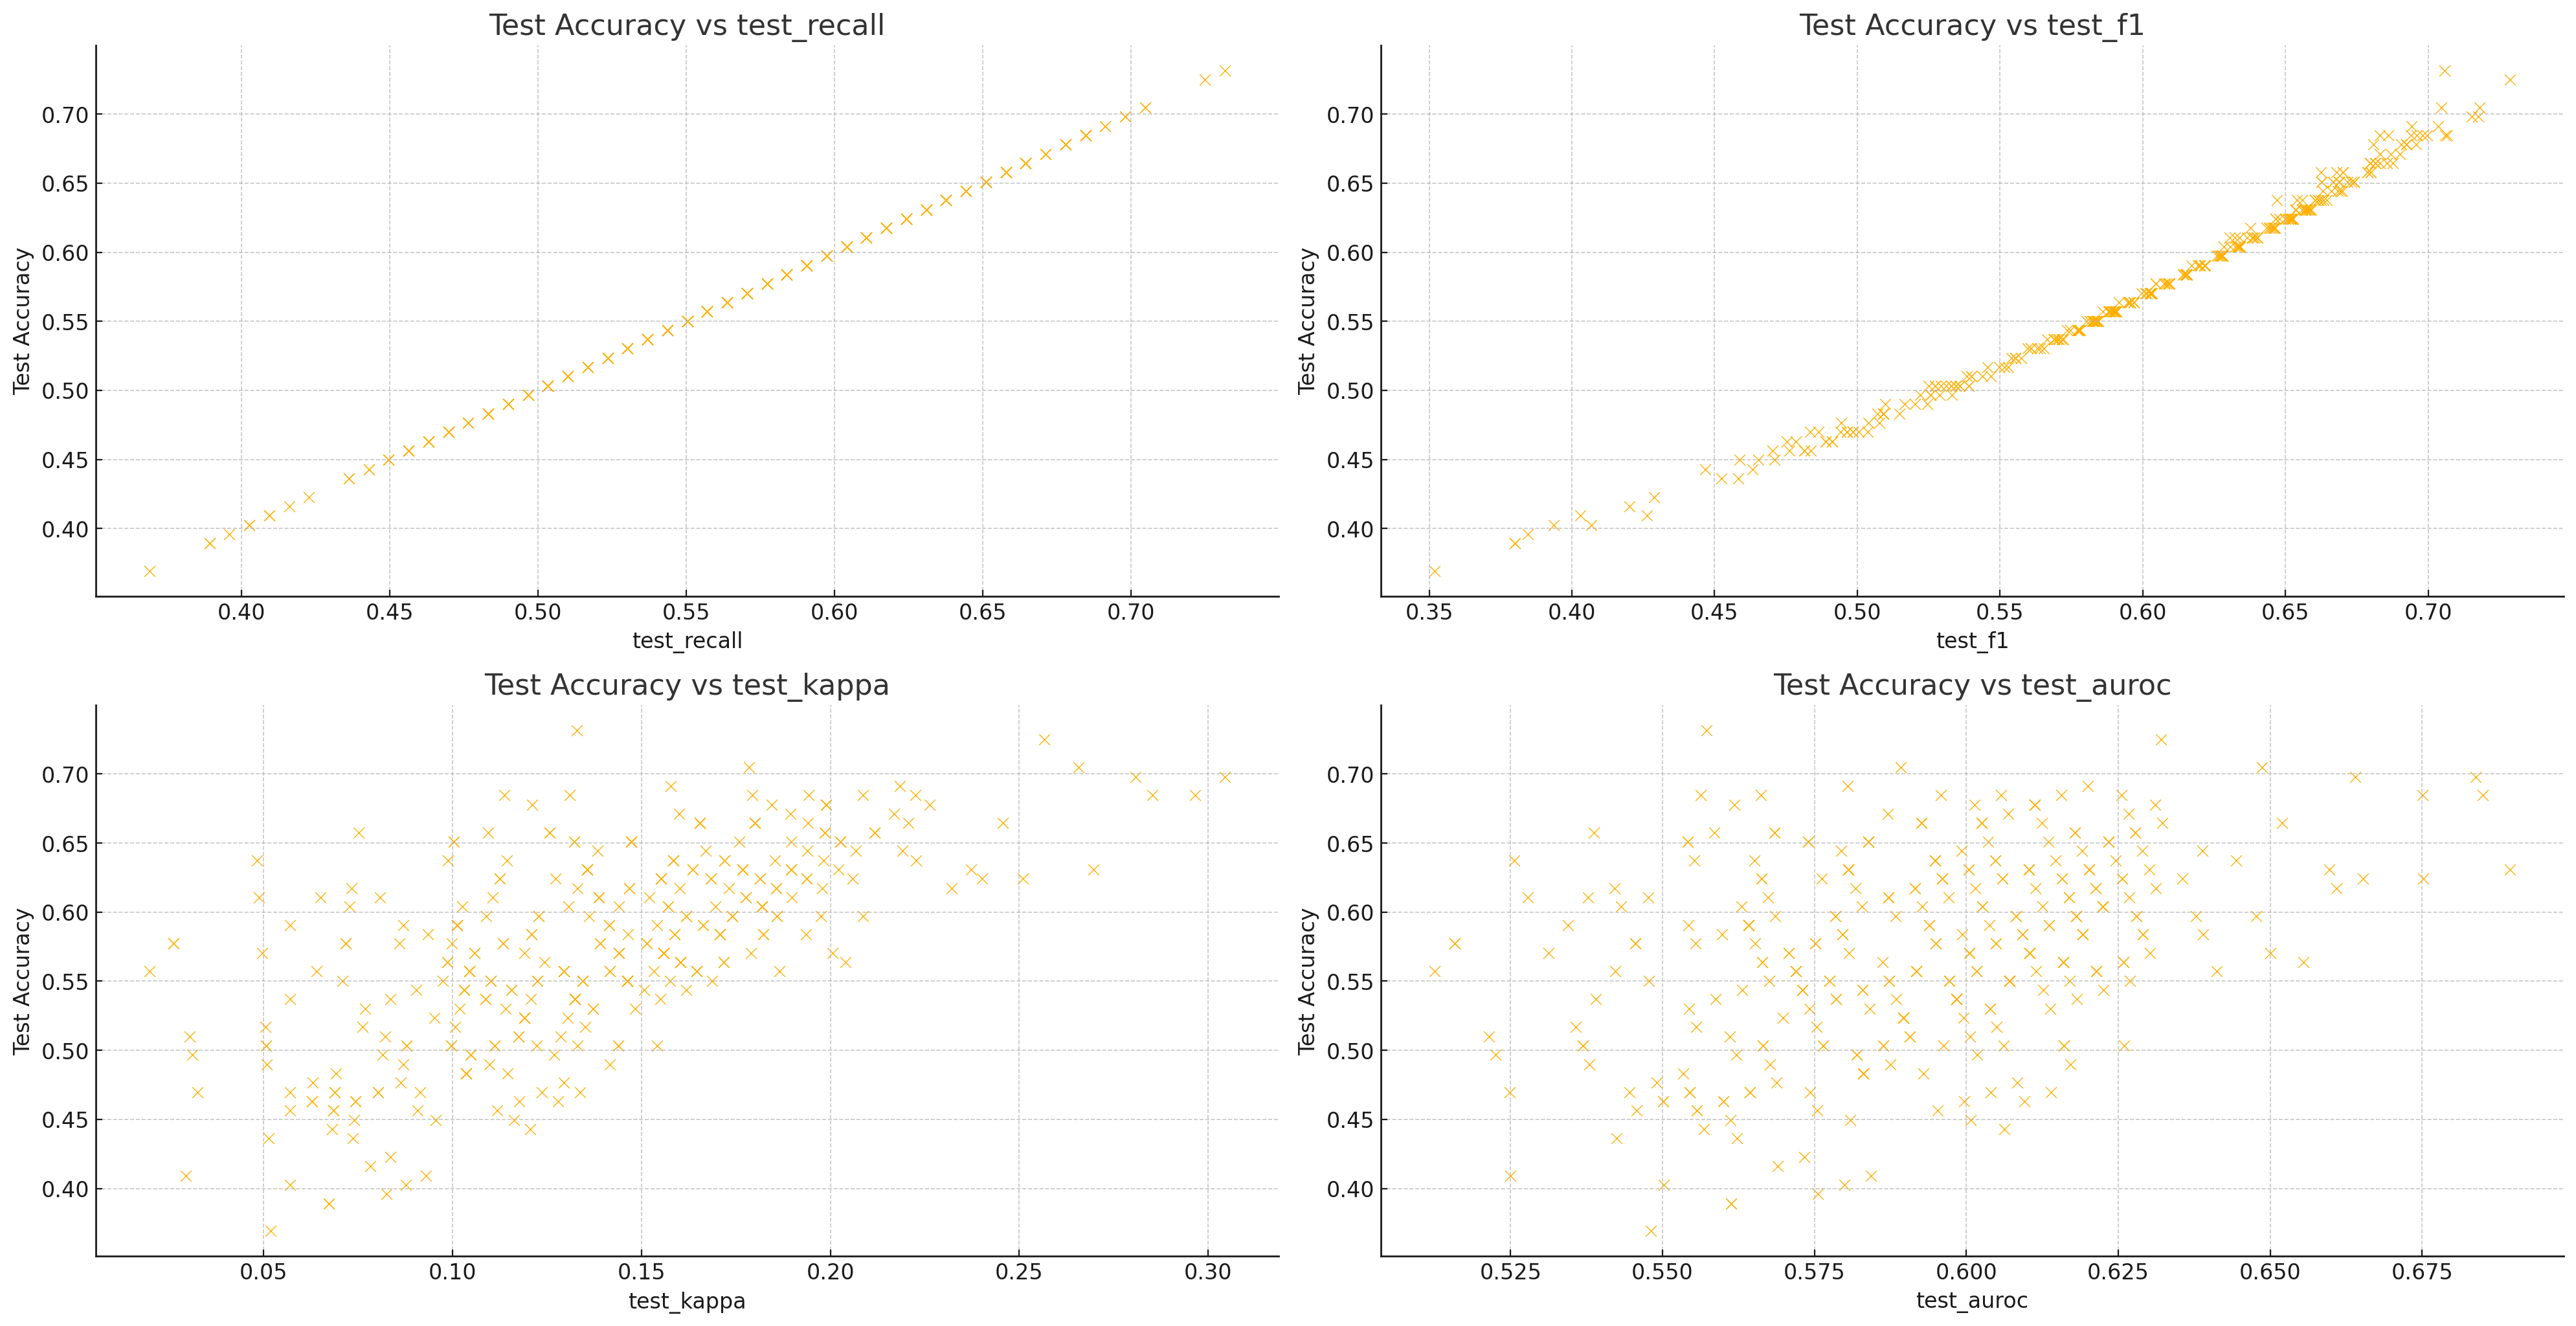
\includegraphics[width=400px]{Figures/results/acc_corr_no_reg.png}
    \caption{Scatter plot of test accuracy's correlation with other metrics for various models.}
    \label{fig: test_corr_no_reg}
\end{figure}

\autoref{fig: test_corr_no_reg_part_1} shows a zoomed-in version of the top left corner of \autoref{fig: test_corr_no_reg}. It shows the correlation between the Accuracy and Recall metrics on the Test set. The diagonal y=x line indicates perfect correlation. The correlation between the two sets is very high.
\begin{figure}[H]
    \centering
    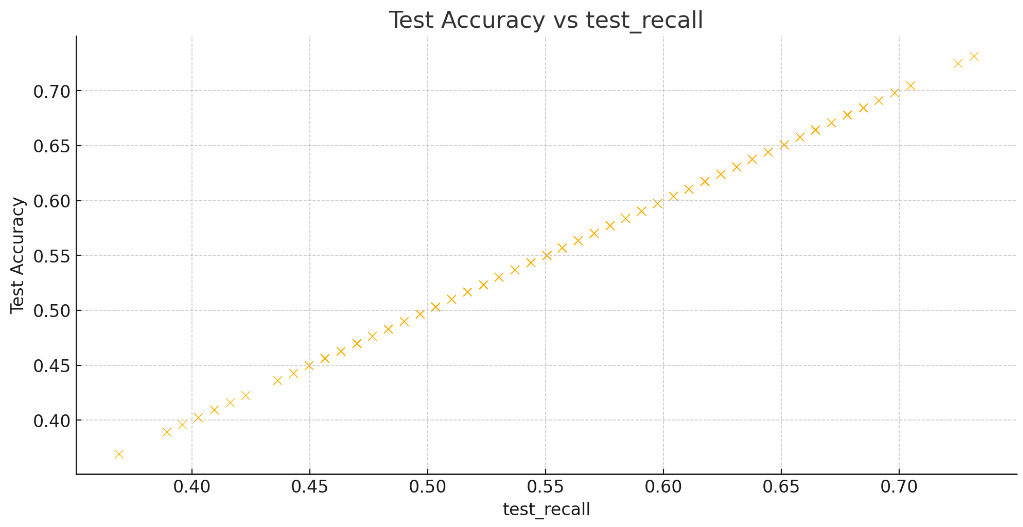
\includegraphics[width=0.9\textwidth]{Figures/results/acc_corr_no_reg_part_1.png}
    \caption{Test Accuracy vs Test Recall.}
    \label{fig: test_corr_no_reg_part_1}
\end{figure}

\autoref{fig: test_corr_no_reg_part_2} shows a zoomed-in version of the top right corner of \autoref{fig: test_corr_no_reg}. It shows the correlation between the Accuracy and F1 metrics on the Test set. The diagonal y=x line indicates perfect correlation. The correlation is lower than in \autoref{fig: test_corr_no_reg_part_1} but still high. The F1 score tends to be higher than the Accuracy, as seen from the points below the y=x line.

\begin{figure}[H]
    \centering
    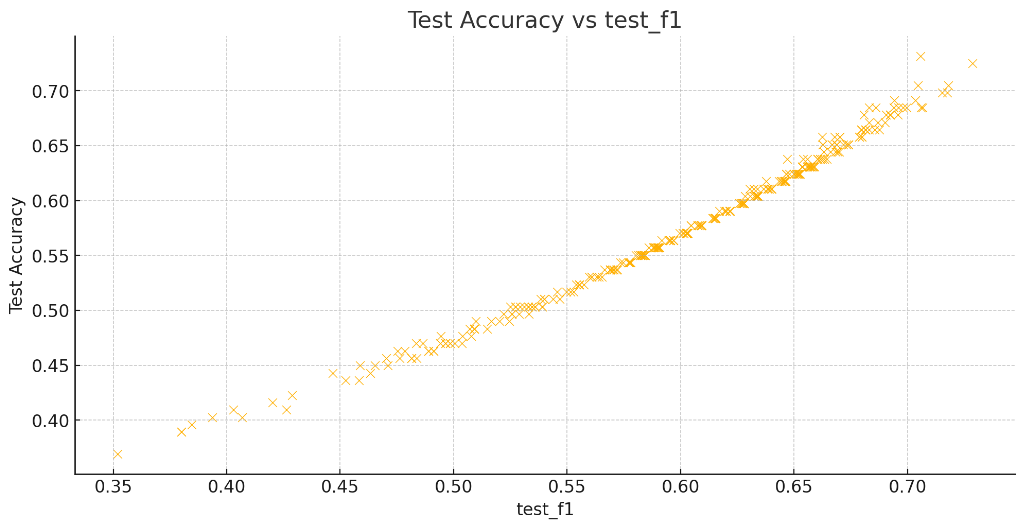
\includegraphics[width=0.9\textwidth]{Figures/results/acc_corr_no_reg_part_2.png}
    \caption{Test Accuracy vs Test F1.}
    \label{fig: test_corr_no_reg_part_2}
\end{figure}

\autoref{fig: test_corr_no_reg_part_3} shows a zoomed-in version of the lower left corner of \autoref{fig: test_corr_no_reg}. It shows the correlation between the Accuracy and Kappa metrics on the Test set. A diagonal line still indicates perfect correlation, but since Kappa's chance value is 0.0 and Accuracy's chance value is 0.5, we expect a bias term of 0.5. From the plot, it's clear that there is a positive correlation between them, but the relationship is less clear than the other plots. A Kappa of 0.05 (barely above chance) has corresponding Accuracy values from about 0.35 (inverted classifier) to about 0.65.

\begin{figure}[H]
    \centering
    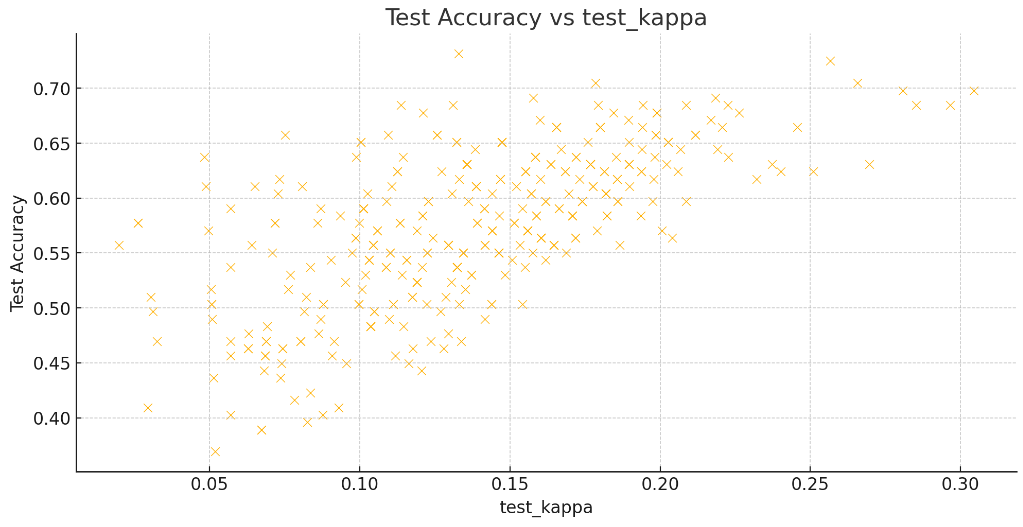
\includegraphics[width=0.9\textwidth]{Figures/results/acc_corr_no_reg_part_3.png}
    \caption{Test Accuracy vs Test Kappa.}
    \label{fig: test_corr_no_reg_part_3}
\end{figure}

\autoref{fig: test_corr_no_reg_part_4} shows a zoomed-in version of the lower right corner of \autoref{fig: test_corr_no_reg}. It shows the correlation between the Accuracy and AUROC metrics on the Test set. A diagonal line still indicates perfect correlation. The plot shows a positive correlation, but the relationship is less clear than in the top plots. 
\begin{figure}[H]
    \centering
    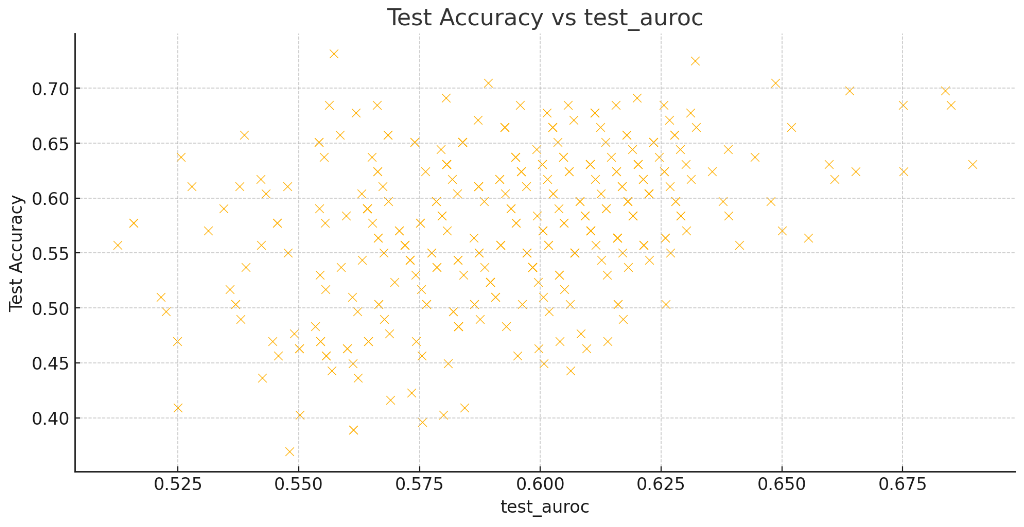
\includegraphics[width=0.9\textwidth]{Figures/results/acc_corr_no_reg_part_4.png}
    \caption{Test Accuracy vs Test AUROC.}
    \label{fig: test_corr_no_reg_part_4}
\end{figure}


\autoref{fig: reg_type_scatter} compares different regularization techniques and the correlation between various sets. Points close to the y=x line indicate a well-adjusted model, while points closer to the training or validation sets indicate overfitting to these sets. L1 and l2 suggest that the L1 and L2 regularization methods were used, respectively, while None means no regularization was applied. Each subplot is plotted below and zoomed in for easy inspection.
\begin{figure}[H]
    \centering
    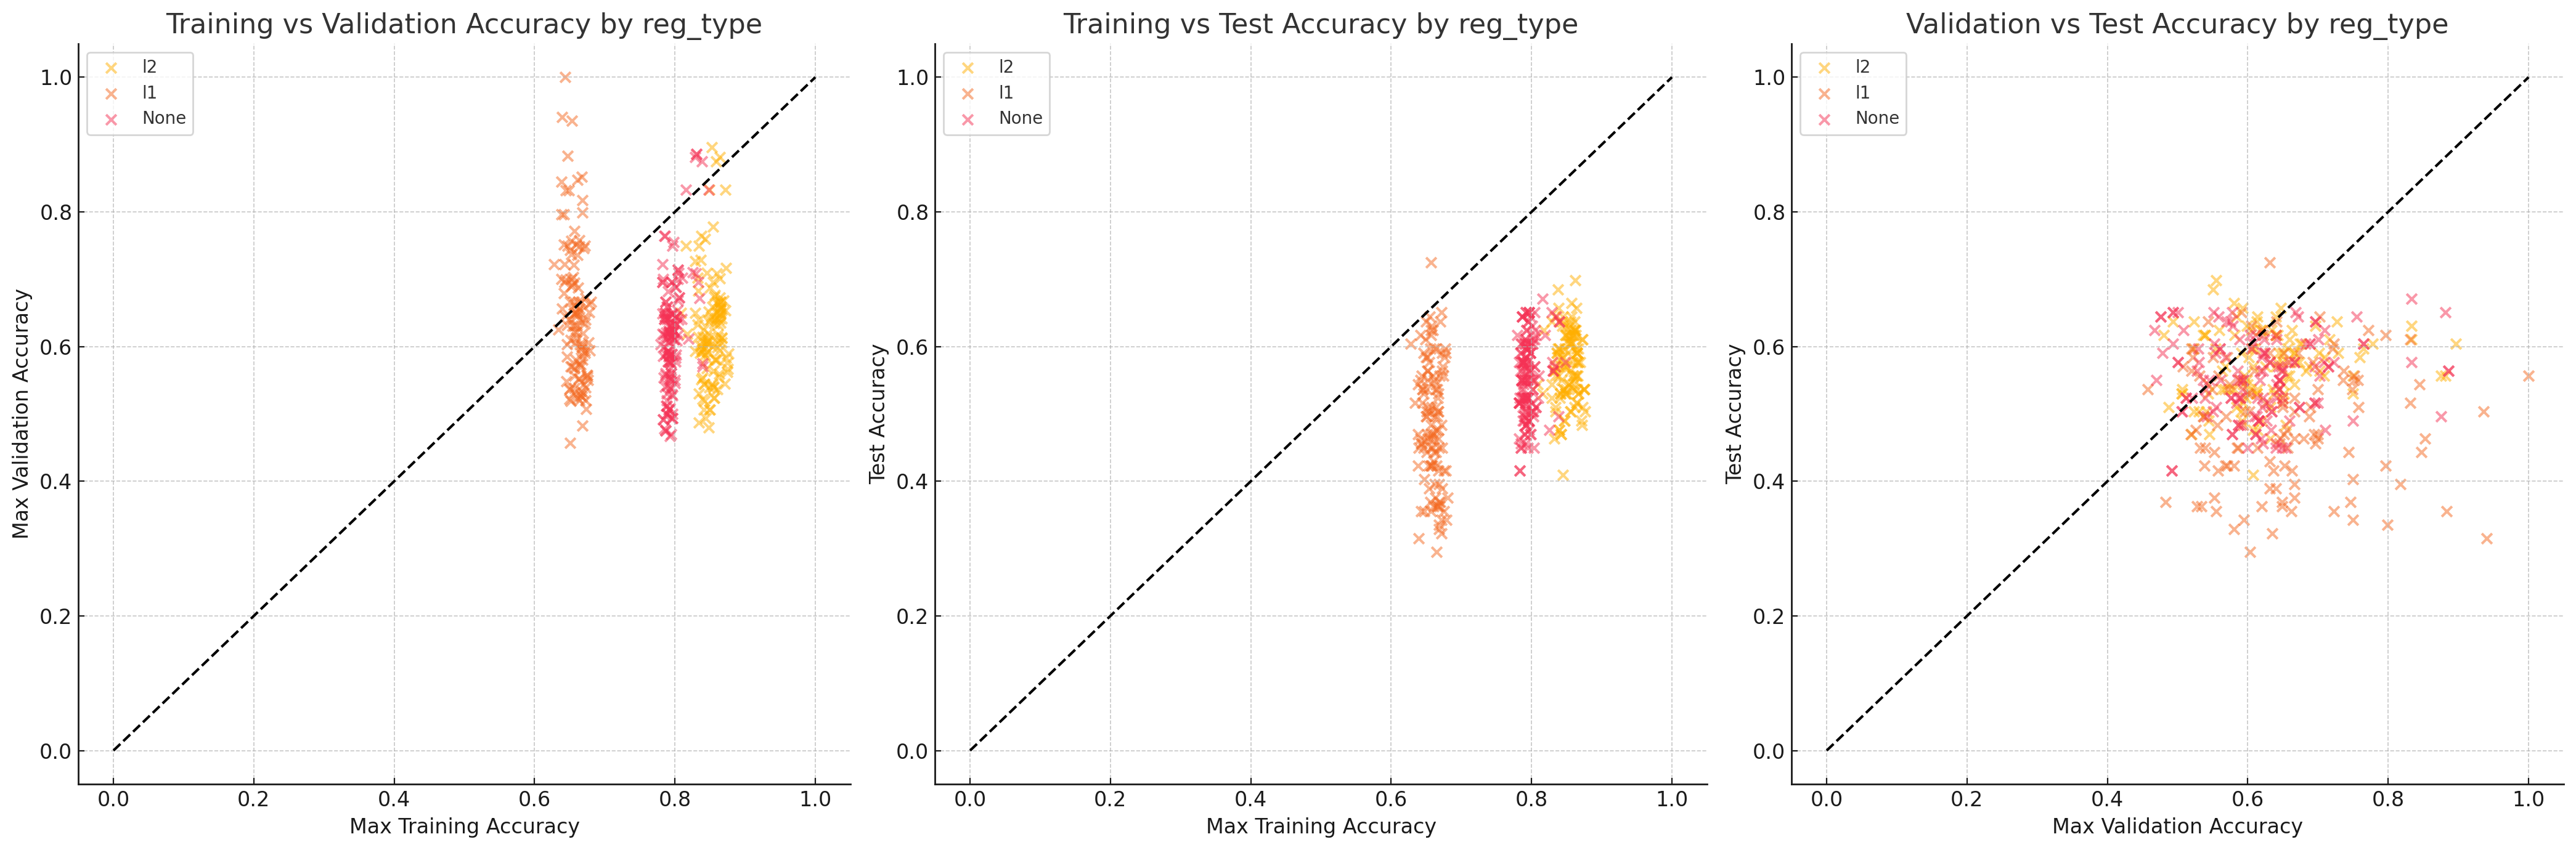
\includegraphics[width=400px]{Figures/results/scatter_reg_type.png}
    \caption{Scatter plot comparing the results of different regularization techniques on the different sets.}
    \label{fig: reg_type_scatter}
\end{figure}

\autoref{fig: reg_type_scatter_part_1} shows a zoomed in version of the left plot in \autoref{fig: reg_type_scatter}. The plot shows every model's highest accuracy score on the training and validation sets collected using their regularization method. A point along the diagonal line indicates an equal score on both sets, meaning the model generalizes well between the sets. A point below the line indicates that the model scored higher on the Training set, while above the line, the score was highest on the Validation set. From the plot, most models scored higher on the Training set. The L1 models never scored above 0.7 on the Training set, and the highest L1 score on the diagonal was just below 0.7. While L2 and None tend to score higher on the Training set, the models scoring highest on the diagonal line scored about 0.85 for L2 and 0.82 for None.

\begin{figure}[H]
    \centering
    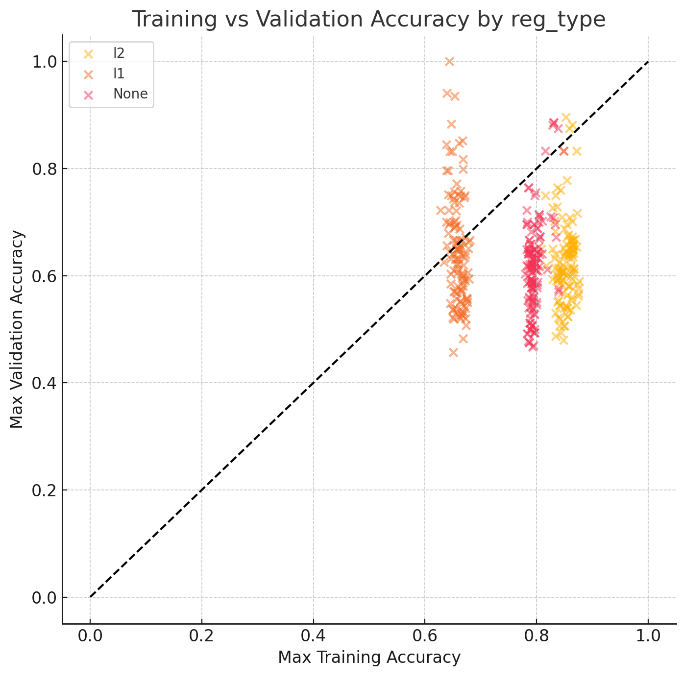
\includegraphics[width=0.7\textwidth]{Figures/results/scatter_reg_type_part_1.png}
    \caption{Training vs Validation Accuracy by reg\_type.}
    \label{fig: reg_type_scatter_part_1}
\end{figure}

\autoref{fig: reg_type_scatter_part_2} shows a zoomed in version of the middle plot in \autoref{fig: reg_type_scatter}. The plot shows every model's highest Accuracy score on the Training and Test sets collected by their regularization method. A point along the diagonal line indicates an equal score on both sets, meaning the model generalizes well between the sets. A point below the line indicates that the model scored higher on the Training set, while above the line, the score was highest on the Test set. From the plot, it's clear that most models scored higher on the Training set, with only one model scoring higher on the Test set. Only the L1 method has some models close to the diagonal. However, they also tend to score lower on both sets.

\begin{figure}[H]
    \centering
    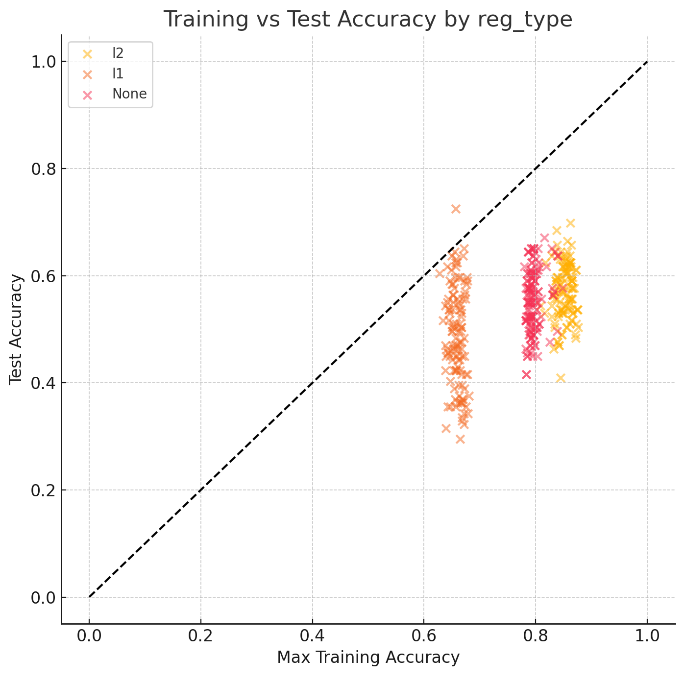
\includegraphics[width=0.7\textwidth]{Figures/results/scatter_reg_type_part_2.png}
    \caption{Training vs Test Accuracy by reg\_type.}
    \label{fig: reg_type_scatter_part_2}
\end{figure}

\autoref{fig: reg_type_scatter_part_3} shows a zoomed in version of the right plot in \autoref{fig: reg_type_scatter}. The plot shows every model's highest Accuracy score on the Validation and Test sets collected by their regularization method. A point along the diagonal line indicates an equal score on both sets, meaning the model generalizes well between the sets. A point below the line indicates that the model scored higher on the Validation set, while above the line, the score was highest on the Test set. From the plot, it's clear that most models scored higher on the Validation set, with only some scoring higher on the Test set. The correlation between the sets is higher than between the Training and Test sets, and the regularization methods are not as clustered. The L1 models are more spread out and tend to score lower on the Test set. The models scoring highest on the diagonal use the None and L2 method, scoring about 0.65.

\begin{figure}[H]
    \centering
    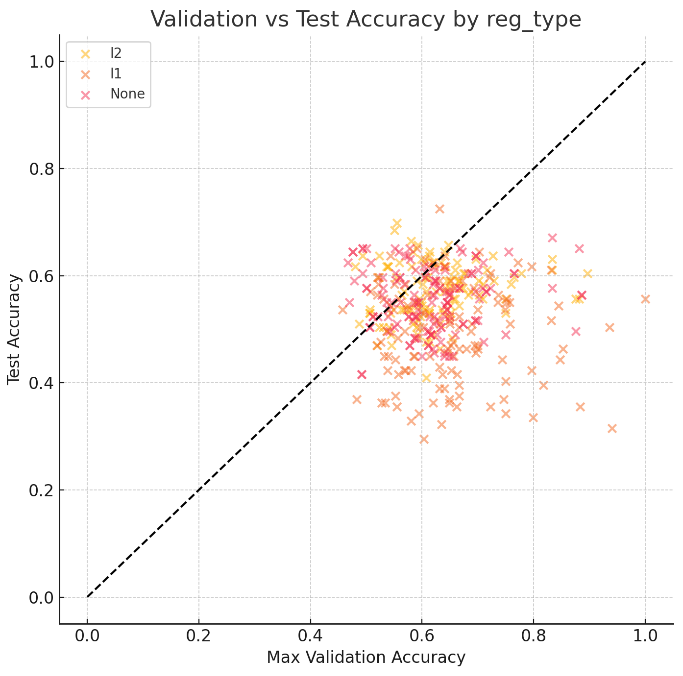
\includegraphics[width=0.7\textwidth]{Figures/results/scatter_reg_type_part_3.png}
    \caption{Validation vs Test Accuracy by reg\_type.}
    \label{fig: reg_type_scatter_part_3}
\end{figure}


\section{Balance Validation Set}
\label{res_sec: balance_val}
The Balance Validation Set parameter is a boolean value that selects whether the Validation set is balanced. A True value means that the Validation set is balanced using undersampling, meaning the majority of class epochs are deleted until there are equally many for both classes. A False value means this undersampling does not happen, and the natural imbalance is maintained in the set. 

In \autoref{fig: balance_val}, the difference statistics between different Balance Validation parameter values are compared on the three sets. On average (indicated by the marker), the False value scores better on the Training and Validation Sets but worse on the Test set for most metrics. The standard deviations (indicated by the vertical lines with short horizontal lines at the caps) seem similar for most metrics to the two parameters. The True parameter value appears to have the highest maximum values (topmost horizontal line) and the lowest minimum values (bottommost horizontal line) for most metrics on most sets.


\begin{figure}[H]
    \centering
    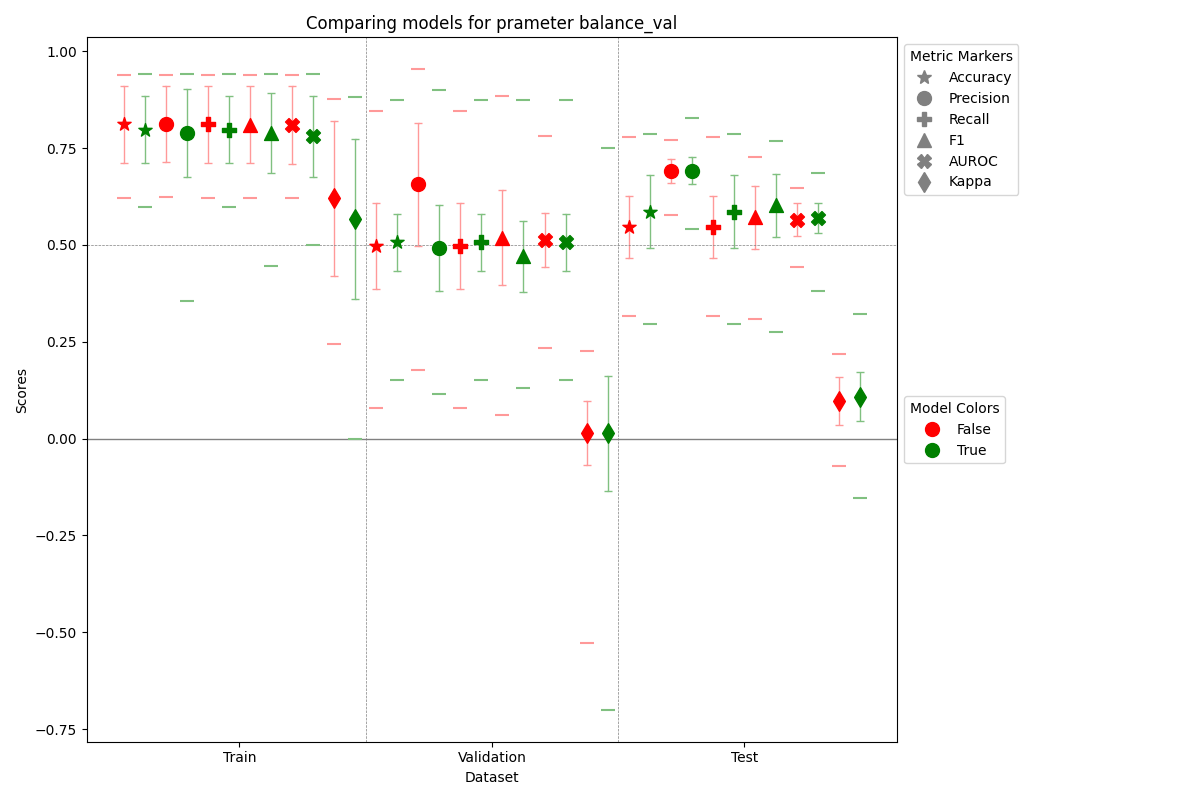
\includegraphics[width=400px]{Figures/results/balance_val/balance_val.png}
    \caption{All models compared by the Balance Validation parameter, a true value signifies an undersampling of the Validation set to have an equal amount of each class.}
    \label{fig: balance_val}
\end{figure}

In \autoref{fig: balance_val_test_auroc}, the Balance Validation parameters are plotted for the models scoring the best on the Test set metric AUROC. This means that there are only two models plotted. The True value model scored significantly better on almost all sets' metrics. The correspondence between the sets is also high, with a low but consistent drop in scores from Training to Validation to Test.


\begin{figure}[H]
    \centering
    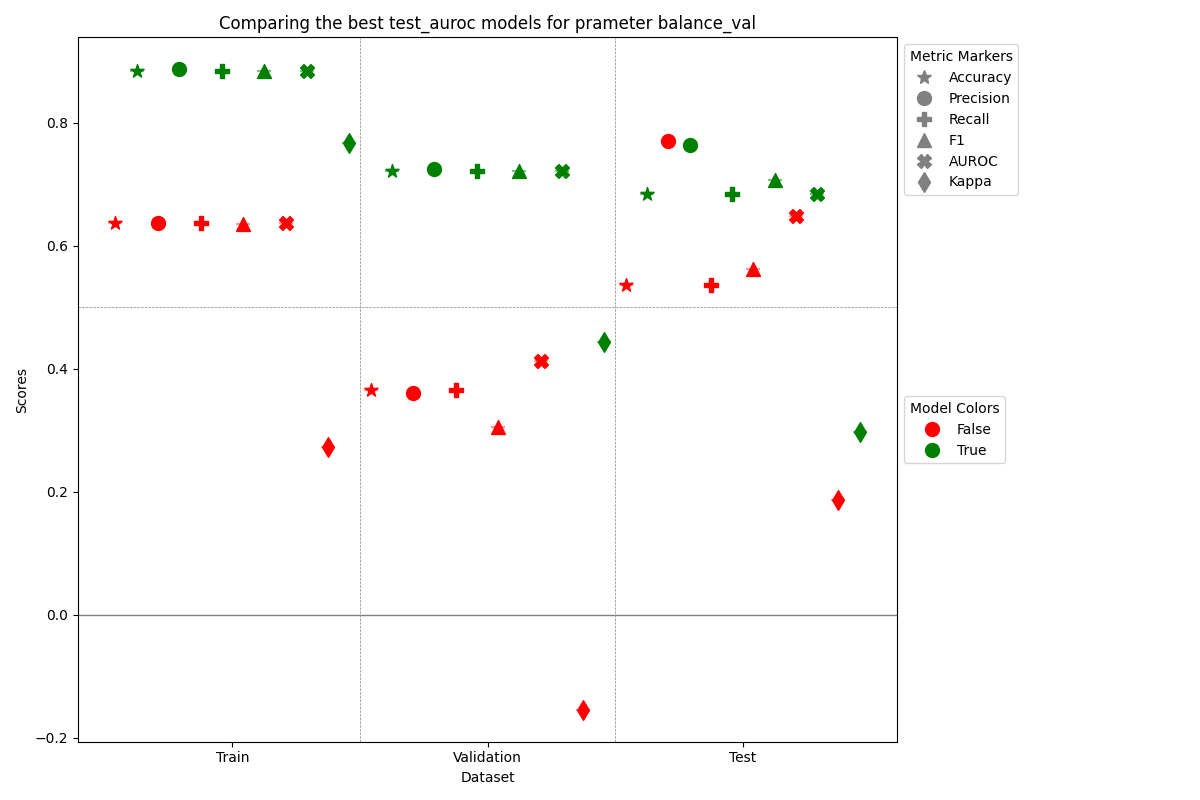
\includegraphics[width=400px]{Figures/results/balance_val/balance_val_test_auroc.png}
    \caption{The best models selected on the Test set AUROC score compared by the Balance Validation parameter.}
    \label{fig: balance_val_test_auroc}
\end{figure}

In \autoref{fig: balance_val_test_kappa}, the Balance Validation parameters are plotted for the models scoring the best on the Test set metric Kappa. This means that there are only two models plotted. The True value model scored better on all metrics on the Test set but worse on all others. The correspondence between the sets is much lower than the model selected through the Test AUROC score. The True valued model scores below chance on the Validation set for all metrics. The False valued model also has low correspondence between the sets. Both models' correspondence between the metrics is high, except for the False valued Kappa score.

\begin{figure}[H]
    \centering
    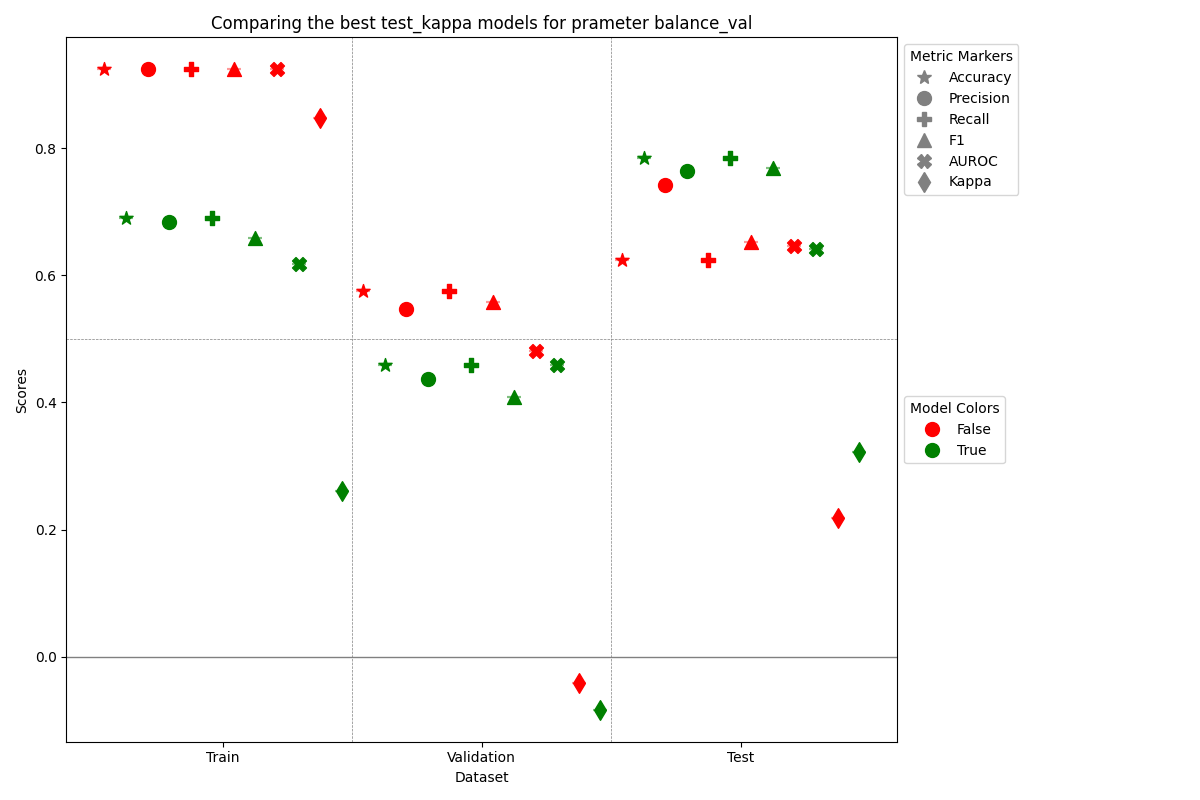
\includegraphics[width=400px]{Figures/results/balance_val/balance_val_test_kappa.png}
    \caption{The best models selected on the Test set Kappa score compared by the Balance Validation parameter.}
    \label{fig: balance_val_test_kappa}
\end{figure}

In \autoref{fig: balance_val_val_auroc}, the Balance Validation parameters are plotted for the models scoring the best on the Validation set metric AUROC. This means that there are only two models plotted. The True value model scored better on most metrics than the False valued model but scored much lower on the Test set than the others. The correspondence between the sets is lower than the model selected through the Test AUROC score. Unlike in \autoref{fig: balance_val_test_kappa}, the True valued models score above chance on all set metrics. The false valued model scores worse overall and is below or at least below the chance level for most of the metrics on the test set.


\begin{figure}[H]
    \centering
    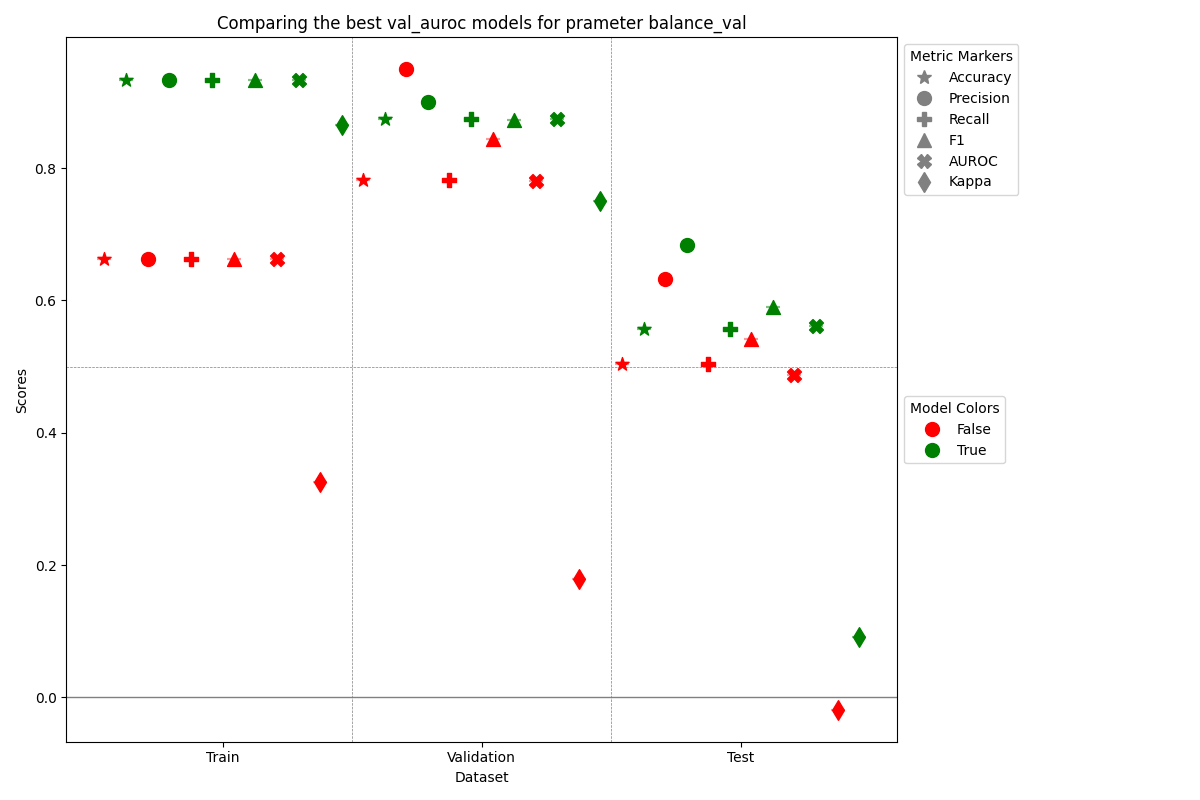
\includegraphics[width=400px]{Figures/results/balance_val/balance_val_val_auroc.png}
    \caption{The best models selected on the Validation set AUROC score compared by the Balance Validation parameter.}
    \label{fig: balance_val_val_auroc}
\end{figure}

In \autoref{fig: balance_val_val_kappa}, the Balance Validation parameters are plotted for the models scoring the best on the Validation set metric Kappa. This means that there are only two models plotted. The True value model scored better on all metrics on all sets than the False valued model. It seems to be the same model as in \autoref{fig: balance_val_val_auroc}. The False valued model has better correspondence between the sets than the False model in \autoref{fig: balance_val_val_auroc} but gets significantly lower scores overall. 


\begin{figure}[H]
    \centering
    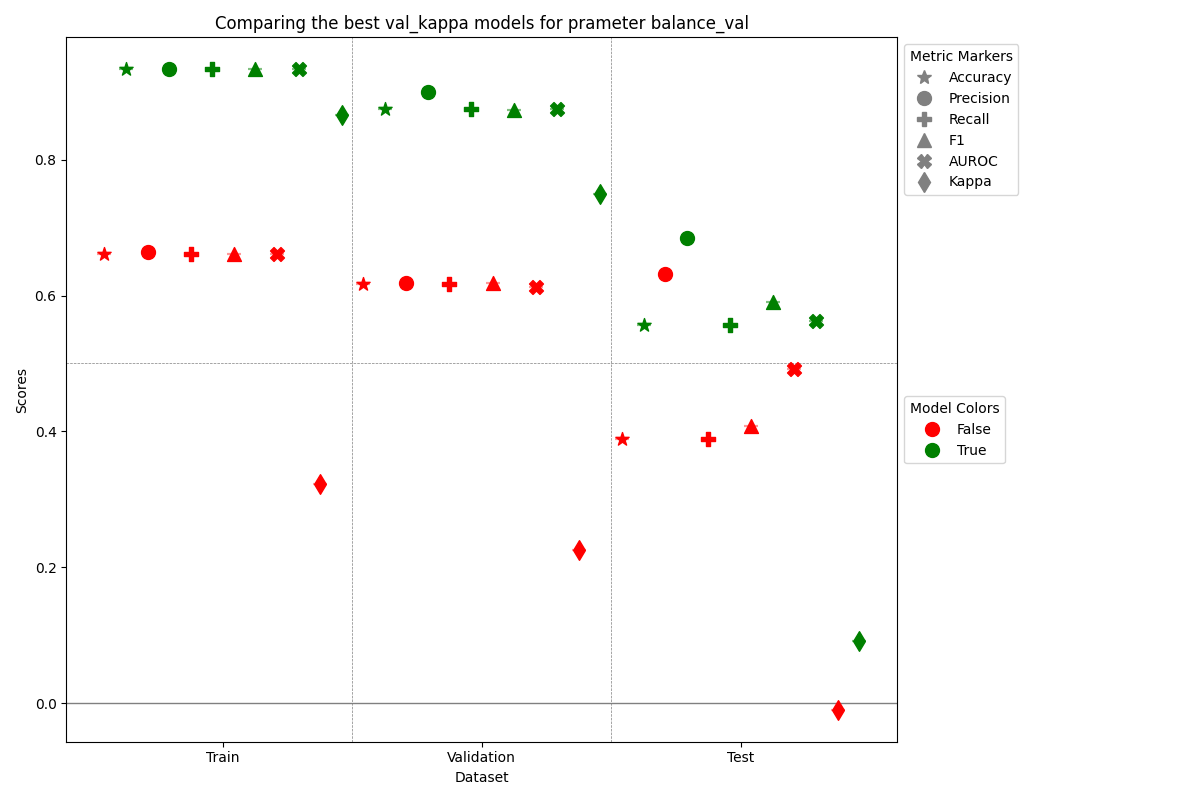
\includegraphics[width=400px]{Figures/results/balance_val/balance_val_val_kappa.png}
    \caption{The best models selected on the Validation set Kappa score compared by the Balance Validation parameter.}
    \label{fig: balance_val_val_kappa}
\end{figure}

\section{MEMD Data Augmentation}
\label{res_sec: memd_data_aug}
The MEMD Data Augmentation parameter is a boolean value used to turn off and on synthetic data generation. A True value signifies synthetic data generated using the MEMD method is added to the dataset, while a False value means no synthetic data is added. From the plots, it seems not using synthetic data is a bit better in the average, while in the best performing models, it's hard to tell if it seems the selection criteria play a more significant role for Test set scores.

In \autoref{fig: memd_data_augmentation_on}, the difference statistics between different MEMD Data Augmentation parameter values are compared on the three sets. On average (indicated by the marker), the False value scores better on the Training and Validation Sets but worse on the Test set for most metrics. The standard deviations (indicated by the vertical lines with short horizontal lines at the caps) seem larger on most metrics for the False value, especially on the Training set. The False parameter value appears to have the highest maximum values (topmost horizontal line) and the lowest minimum values (bottommost horizontal line) for all metrics in most sets.

\begin{figure}[H]
    \centering
    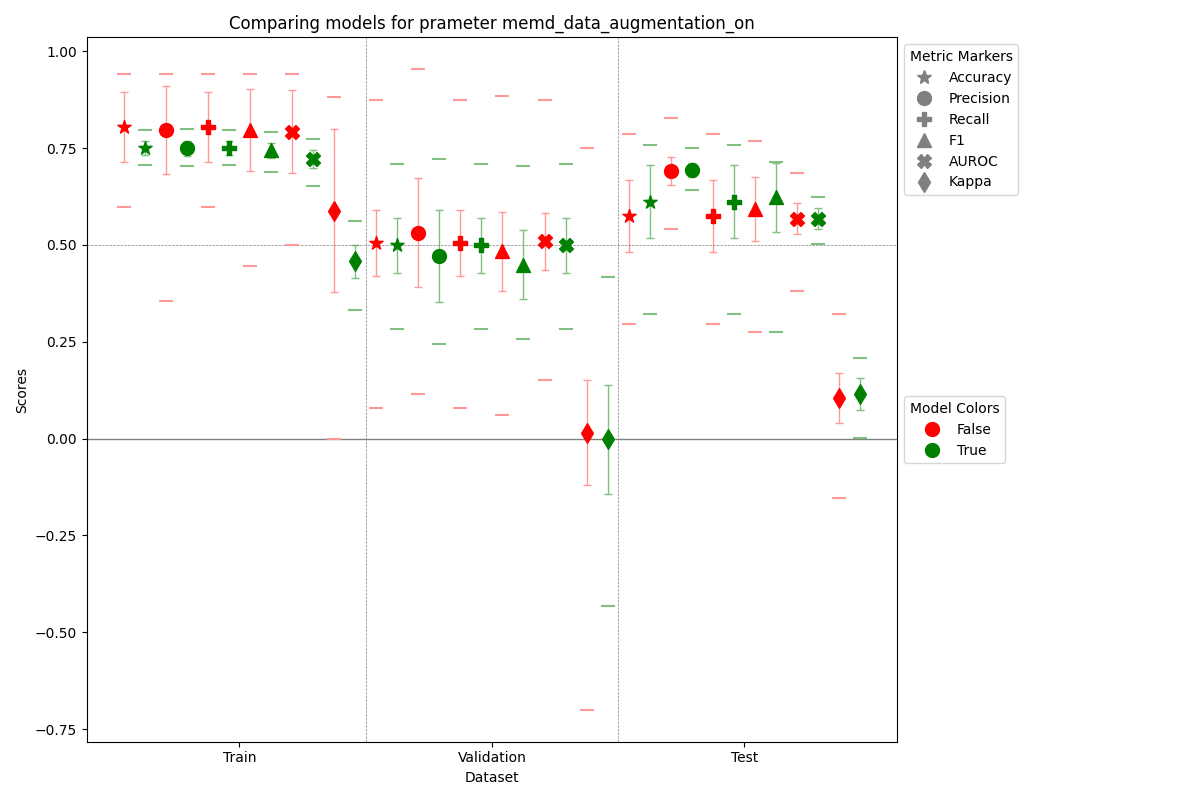
\includegraphics[width=400px]{Figures/results/memd_data_augmentation_on/memd_data_augmentation_on.png}
    \caption{All models compared by the MEMD Data Augmentation parameter, a True value signifies synthetic data generation using the MEMD method while a False value means no synthetic data.}
    \label{fig: memd_data_augmentation_on}
\end{figure}

In \autoref{fig: memd_data_augmentation_on_test_auroc}, the MEMD Data Augmentation parameters are plotted for the models scoring the best on the Test set metric AUROC. This means that there are only two models plotted. The False value model scored significantly better on all metrics on all sets. The correspondence between the sets is also high, with a low but consistent drop in scores from Training to Validation to Test.


\begin{figure}[H]
    \centering
    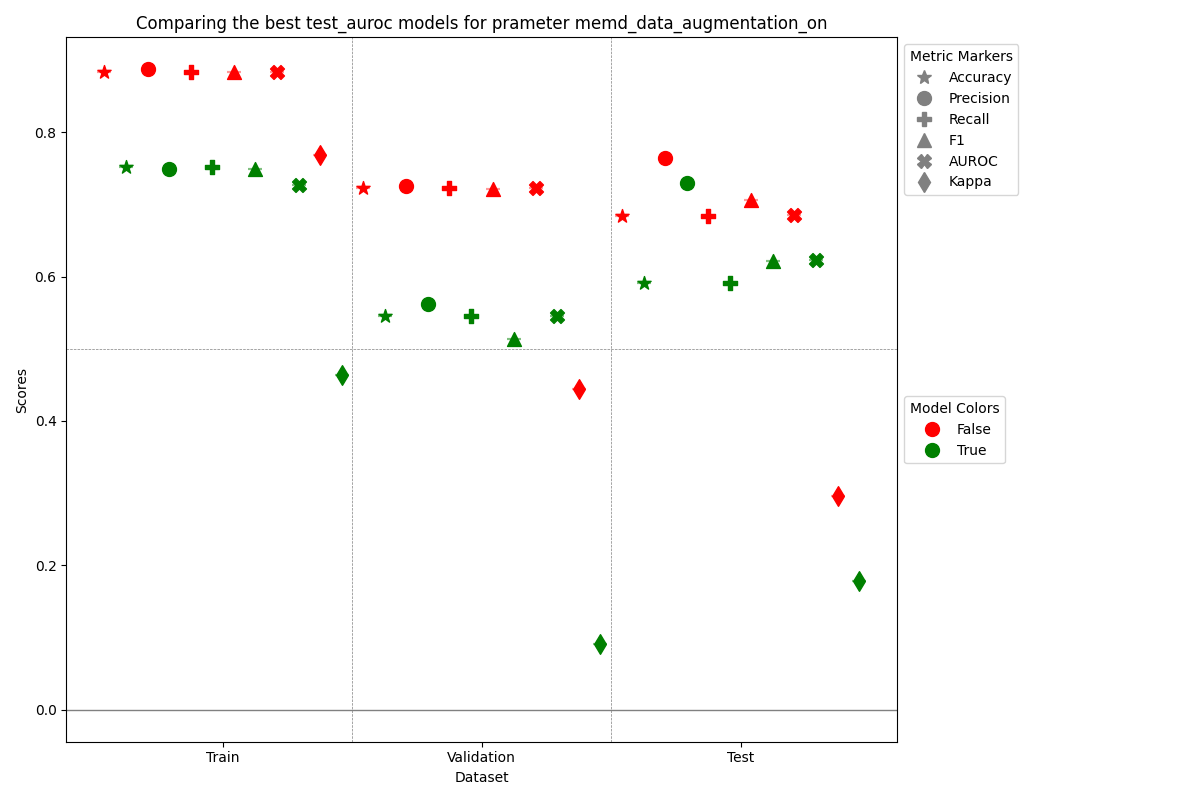
\includegraphics[width=400px]{Figures/results/memd_data_augmentation_on/memd_data_augmentation_on_test_auroc.png}
    \caption{The best models selected on the Test set AUROC score compared by the MEMD Data Augmentation parameter.}
    \label{fig: memd_data_augmentation_on_test_auroc}
\end{figure}

In \autoref{fig: memd_data_augmentation_on_test_kappa}, the MEMD Data Augmentation parameters are plotted for the best models scoring on the Test set metric Kappa. This means that there are only two models plotted. The False value model scored better on all metrics on the Test set but worse on all others. The correspondence between the sets is much lower than the model selected through the Test AUROC score. The False valued model scores below chance on the Validation set for all metrics. The True valued model also has low correspondence between the sets but is better than the False. The correspondence between the metrics is high for both models.

\begin{figure}[H]
    \centering
    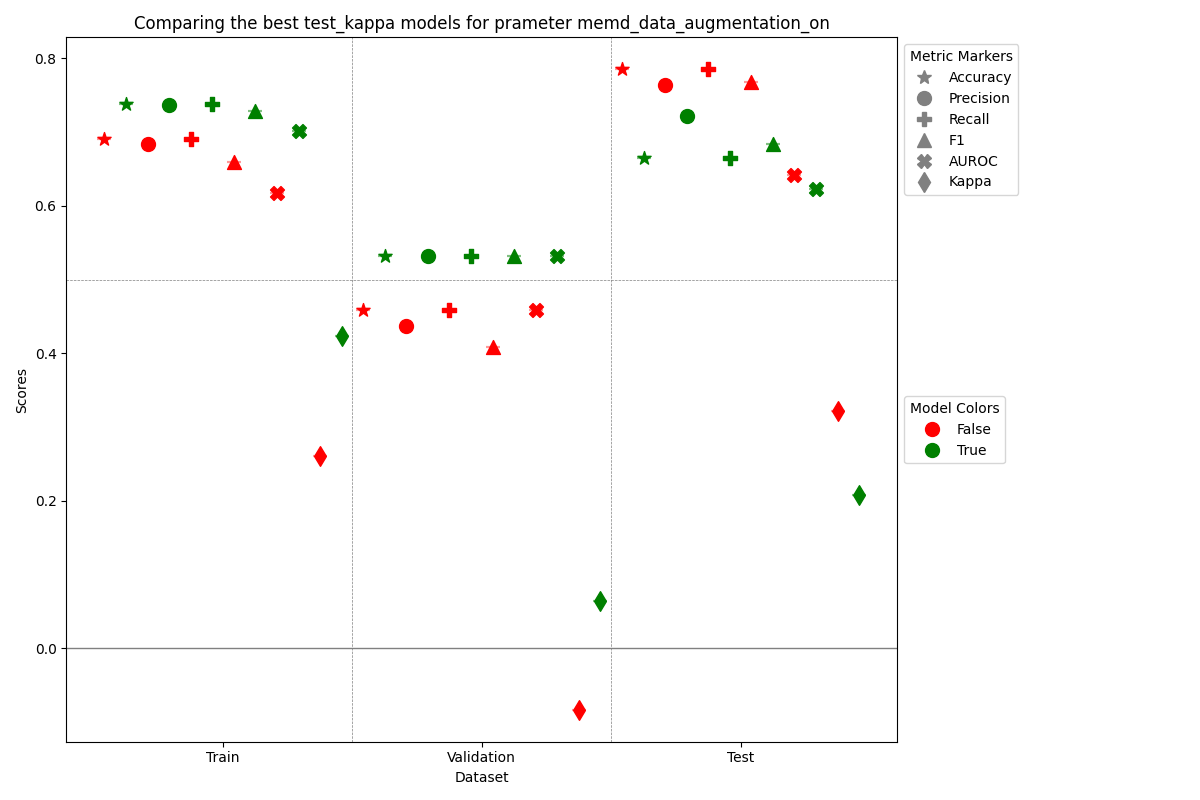
\includegraphics[width=400px]{Figures/results/memd_data_augmentation_on/memd_data_augmentation_on_test_kappa.png}
    \caption{The best models selected on the Test set Kappa score compared by the MEMD Data Augmentation parameter.}
    \label{fig: memd_data_augmentation_on_test_kappa}
\end{figure}

In \autoref{fig: memd_data_augmentation_on_val_auroc}, the MEMD Data Augmentation parameters are plotted for the models scoring the best on the Validation set metric AUROC. This means that there are only two models plotted. The False value model scored better on all metrics on the Training and Validation sets than the True valued model but scored significantly lower on the Test set than the other sets and worse than the True valued model. The correspondence between the sets is similar to the model selected through the Test AUROC score. Unlike in \autoref{fig: memd_data_augmentation_on_test_kappa}, the False valued models score above chance on all metrics on all sets. The True valued model scores better on the Test set and has higher correspondence between the sets.


\begin{figure}[H]
    \centering
    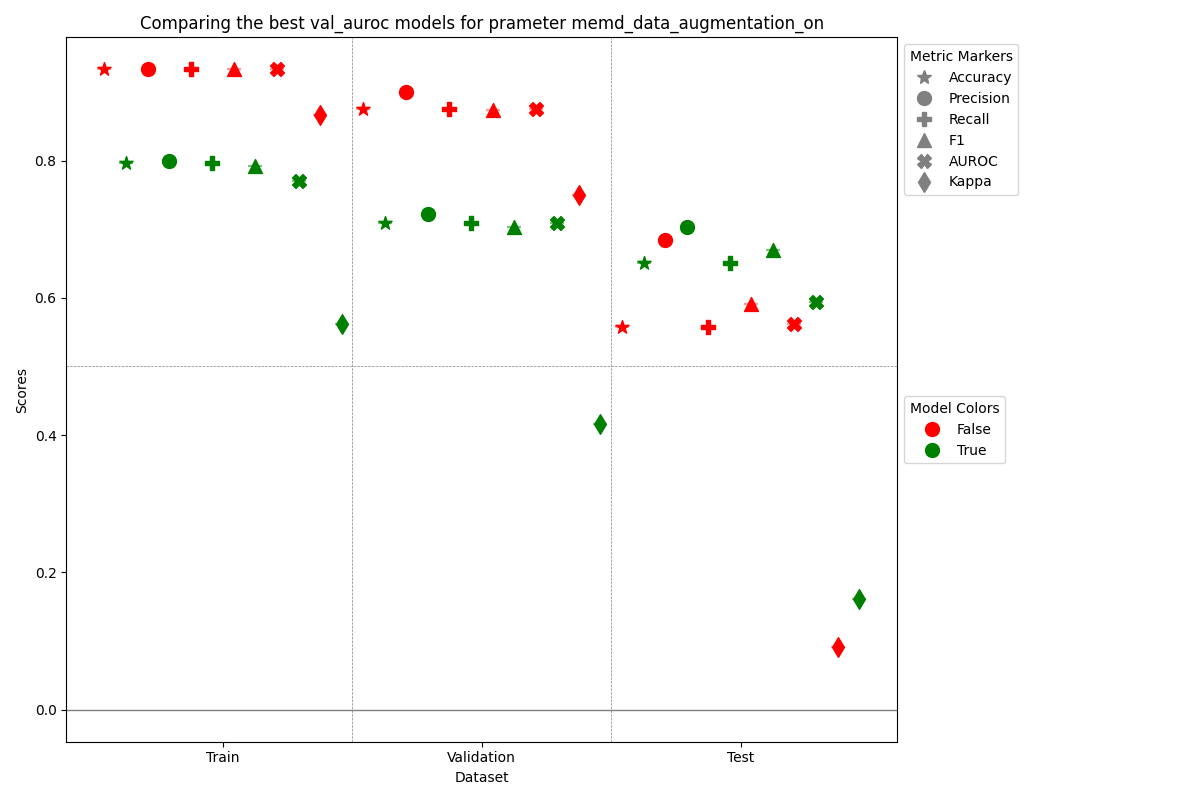
\includegraphics[width=400px]{Figures/results/memd_data_augmentation_on/memd_data_augmentation_on_val_auroc.png}
    \caption{The best models selected on the Validation set AUROC score compared by the MEMD Data Augmentation parameter.}
    \label{fig: memd_data_augmentation_on_val_auroc}
\end{figure}

In \autoref{fig: memd_data_augmentation_on_val_kappa}, the MEMD Data Augmentation parameters are plotted for the models scoring the best on the Validation set metric Kappa. It seems to be the same models selected as in \autoref{fig: memd_data_augmentation_on_val_auroc}, meaning both models were the best on both Kappa and AUROC on the Validation set.

\begin{figure}[H]
    \centering
    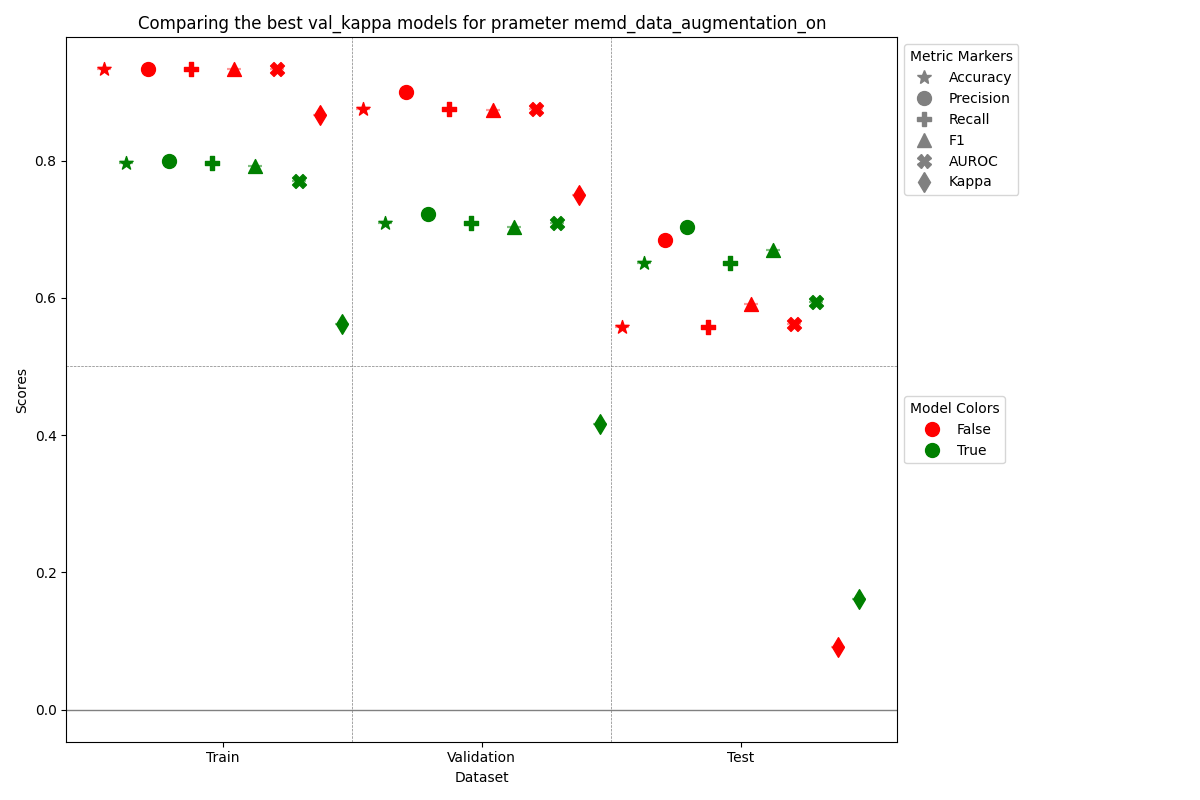
\includegraphics[width=400px]{Figures/results/memd_data_augmentation_on/memd_data_augmentation_on_val_kappa.png}
    \caption{The best models selected on the Validation set Kappa score compared by the MEMD Data Augmentation parameter.}
    \label{fig: memd_data_augmentation_on_val_kappa}
\end{figure}


\section{MEMD Ratio}
\label{res_sec: memd_ratio}
The MEMD Ratio parameter is a floating point value that signifies the ratio of the real data length to be generated synthetically using the MEMD method. A higher value means more synthetic data is generated and added to the Training set. A ratio of 1.0 means 50\% of the total training data is artificial, as explained in \autoref{subsec: augmentation_ratio}. It's essential to keep in mind that these values are only significant. 

As in \autoref{res_sec: balance_val} and \autoref{res_sec: memd_data_aug}, the correspondence between sets was best for the models scoring the best on the Test set using the metric AUROC. Also, like in \autoref{res_sec: memd_data_aug}, the same models scored the best on the metrics Kappa and AUROC on the Validation set. Due to this and the similarity of all parameter values, these plots have been left out.

In \autoref{fig: memd_ratio}, the difference statistics between different MEMD Ratio parameter values are compared on the three sets. It's hard to see the individual ratios due to the amount of metrics and parameter values plotted. However, this is chosen to showcase how similar these values are for all ratios. The data has been filtered to only use models with the MEMD Augmentation turned on to not skew the data since the Ratio parameter has no effect when turned off.

\begin{figure}[H]
    \centering
    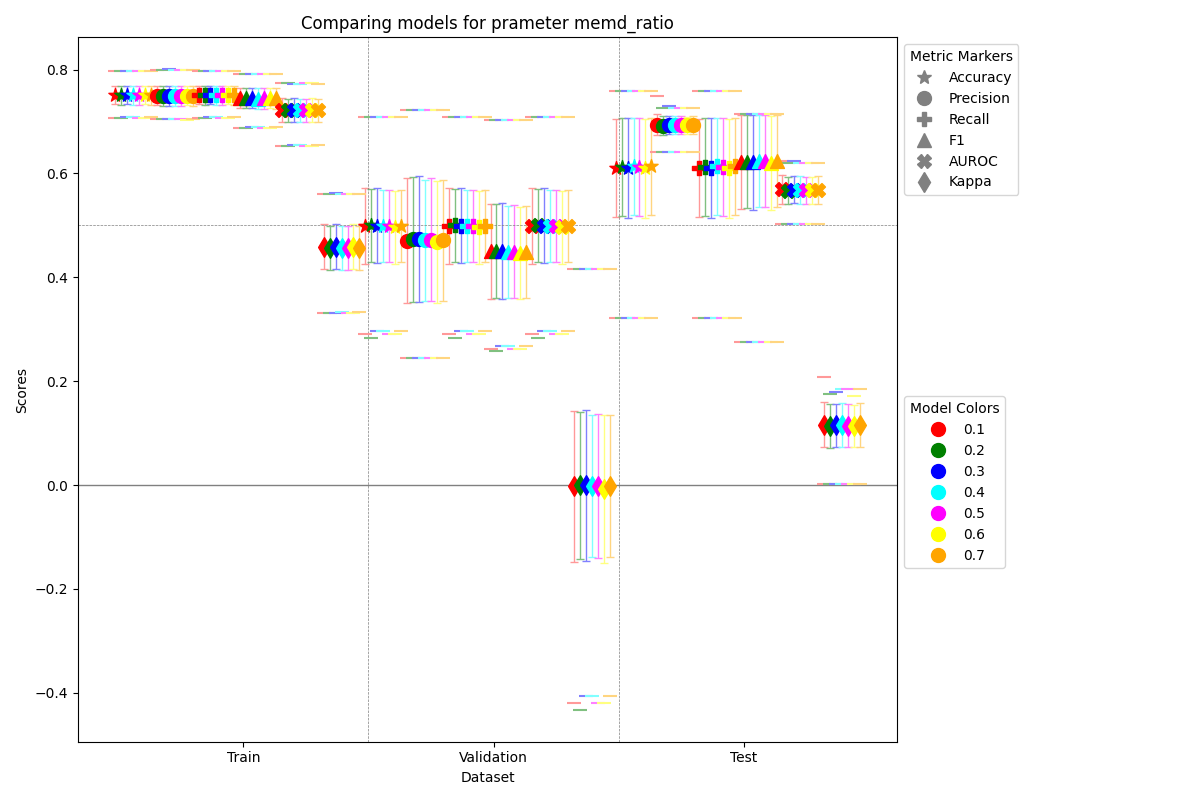
\includegraphics[width=400px]{Figures/results/memd_ratio/memd_ratio.png}
    \caption{All models compared by the MEMD Ratio parameter signifies the ratio of the real data length to be generated synthetically using the MEMD method. }
    \label{fig: memd_ratio}
\end{figure}
\begin{comment}
\begin{figure}[H]
    \centering
    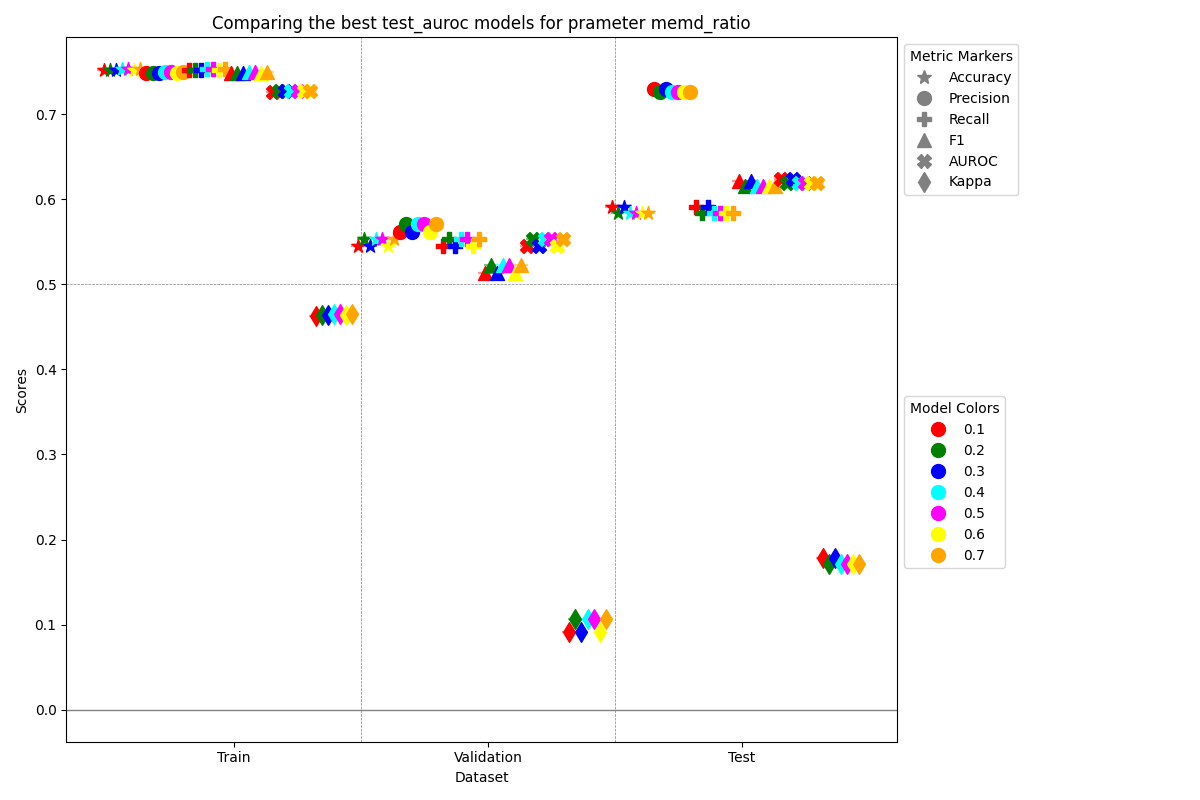
\includegraphics[width=400px]{Figures/results/memd_ratio/memd_ratio_test_auroc.png}
    \caption{The best models selected on the Test set AUROC score compared by the MEMD Ratio parameter.}
    \label{fig: memd_ratio_test_auroc}
\end{figure}


\begin{figure}[H]
    \centering
    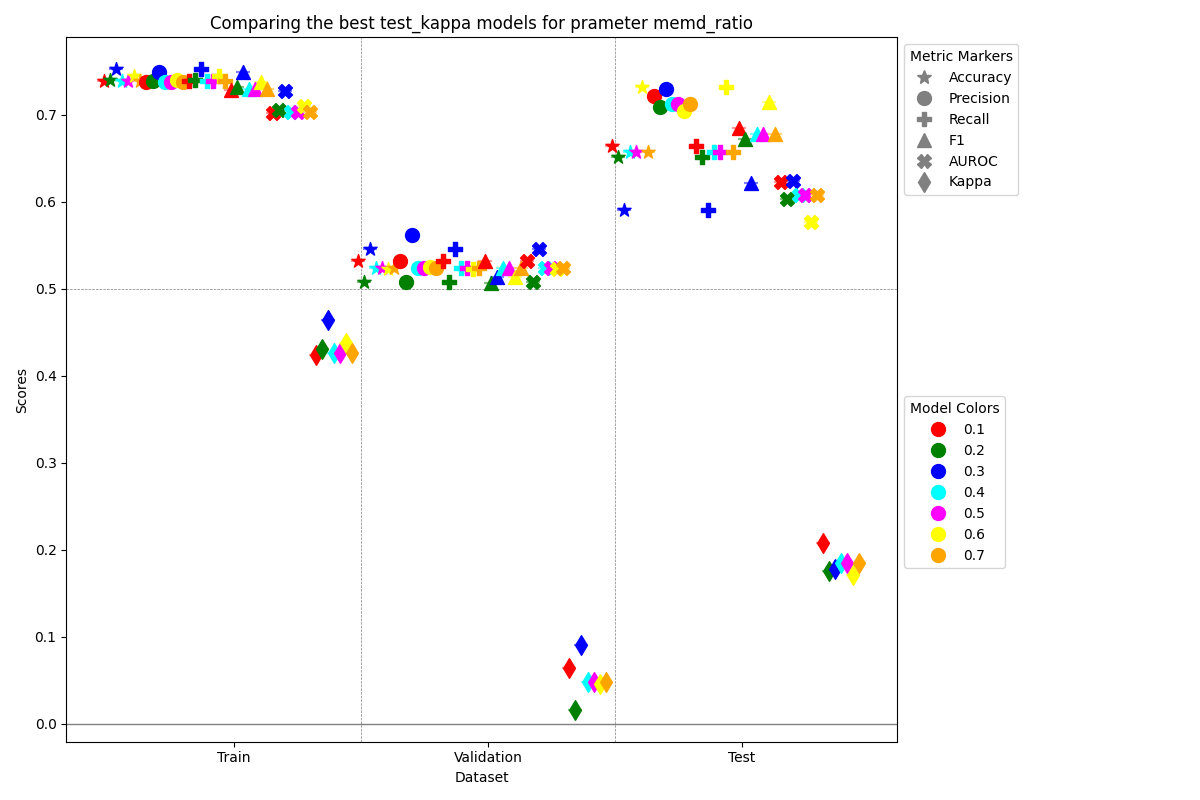
\includegraphics[width=400px]{Figures/results/memd_ratio/memd_ratio_test_kappa.png}
    \caption{The best models selected on the Test set Kappa score compared by the MEMD Ratio parameter.}
    \label{fig: memd_ratio_test_kappa}
\end{figure}

\begin{figure}[H]
    \centering
    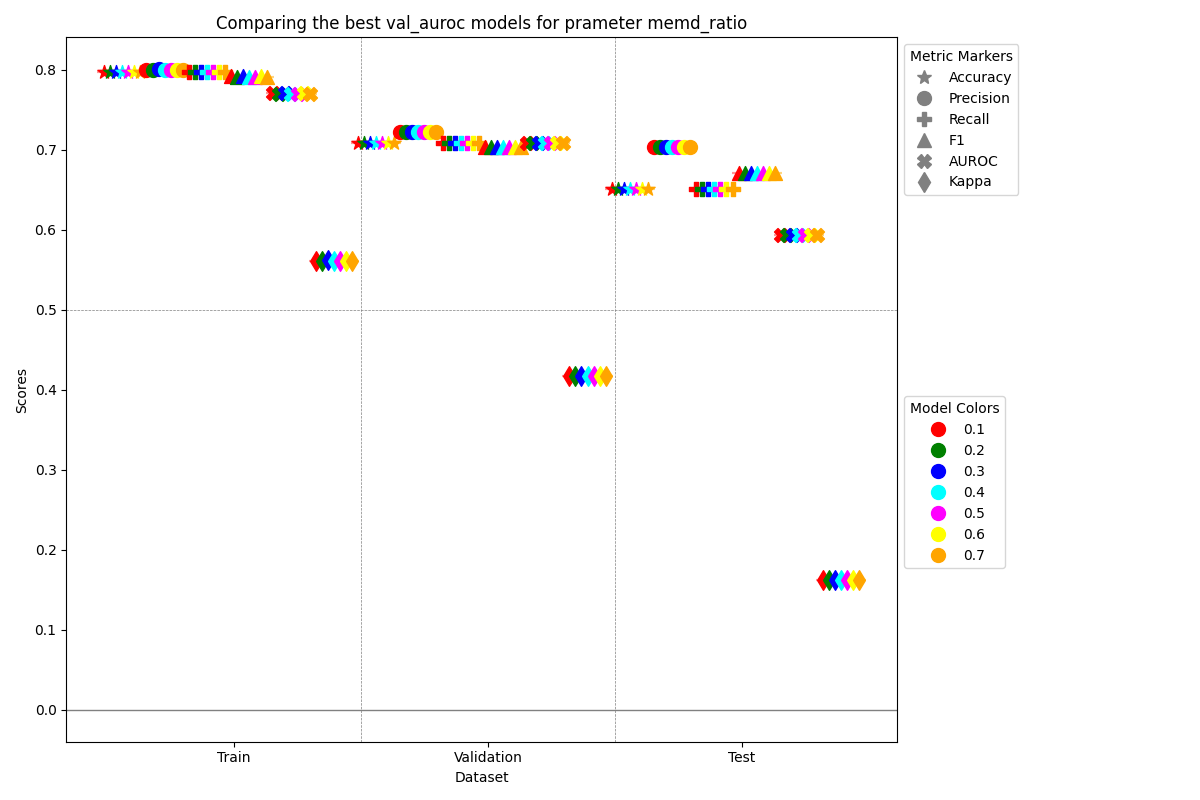
\includegraphics[width=400px]{Figures/results/memd_ratio/memd_ratio_val_auroc.png}
    \caption{The best models selected on the Validation set AUROC score compared by the MEMD Ratio parameter.}
    \label{fig: memd_ratio_val_auroc}
\end{figure}

\begin{figure}[H]
    \centering
    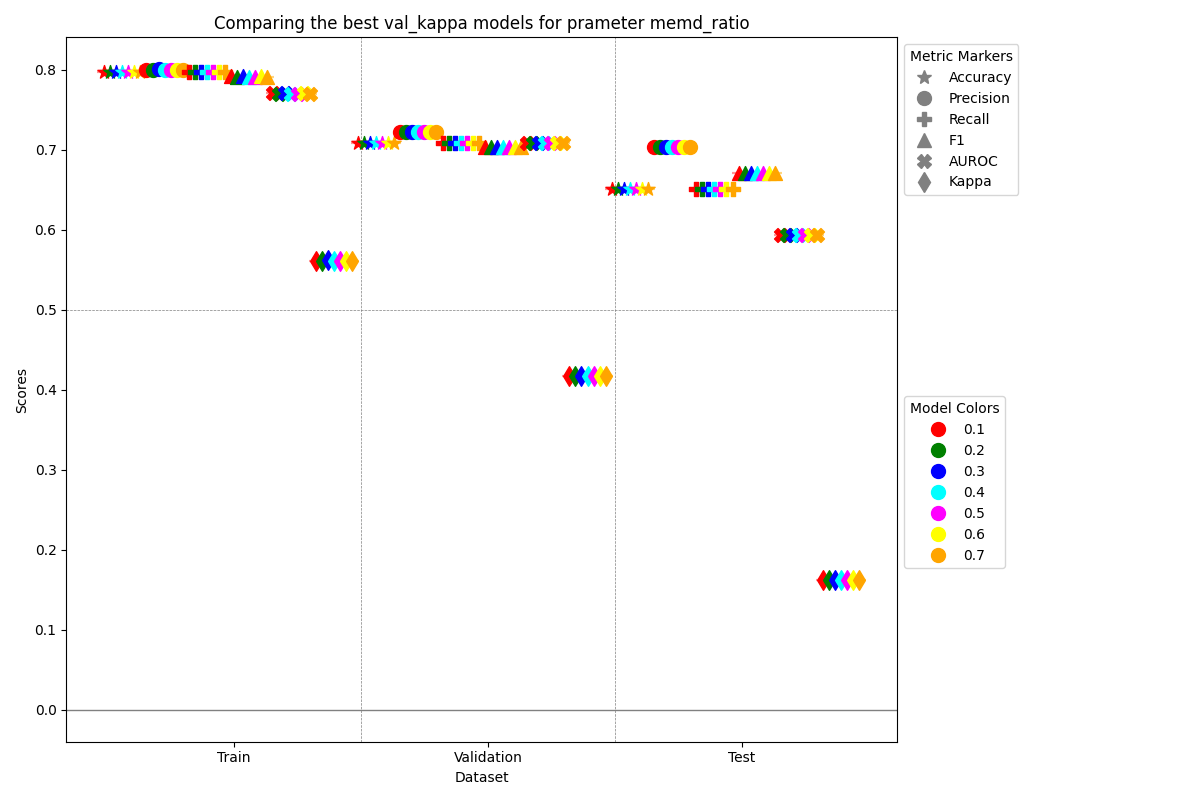
\includegraphics[width=400px]{Figures/results/memd_ratio/memd_ratio_val_kappa.png}
    \caption{The best models selected on the Validation set Kappa score compared by the MEMD Ratio parameter.}
    \label{fig: memd_ratio_val_kappa}
\end{figure}
\end{comment}


\section{IMF Cleaning}
The IMF Cleaning parameter is an integer or None value. A None value signifies no cleaning is done, and the raw signal is passed to the classifier. An integer value means the number of IMFs kept in the cleaned signal after sorting for importance, as explained in 
\autoref{subsec: img_selection}.

For similar reasons as in \autoref{res_sec: memd_ratio}, only the statistics plot and the models scoring the best on the Test set using the metric AUROC will be displayed in the results. 

In \autoref{fig: memd_ratio}, the difference statistics between different IMF Cleaning parameter values are compared on the three sets. Similarly to \autoref{res_sec: memd_ratio}, it is hard to see the individual values due to the number of metrics and parameter values plotted. However, this is chosen to showcase how similar these values are. 

\begin{figure}[H]
    \centering
    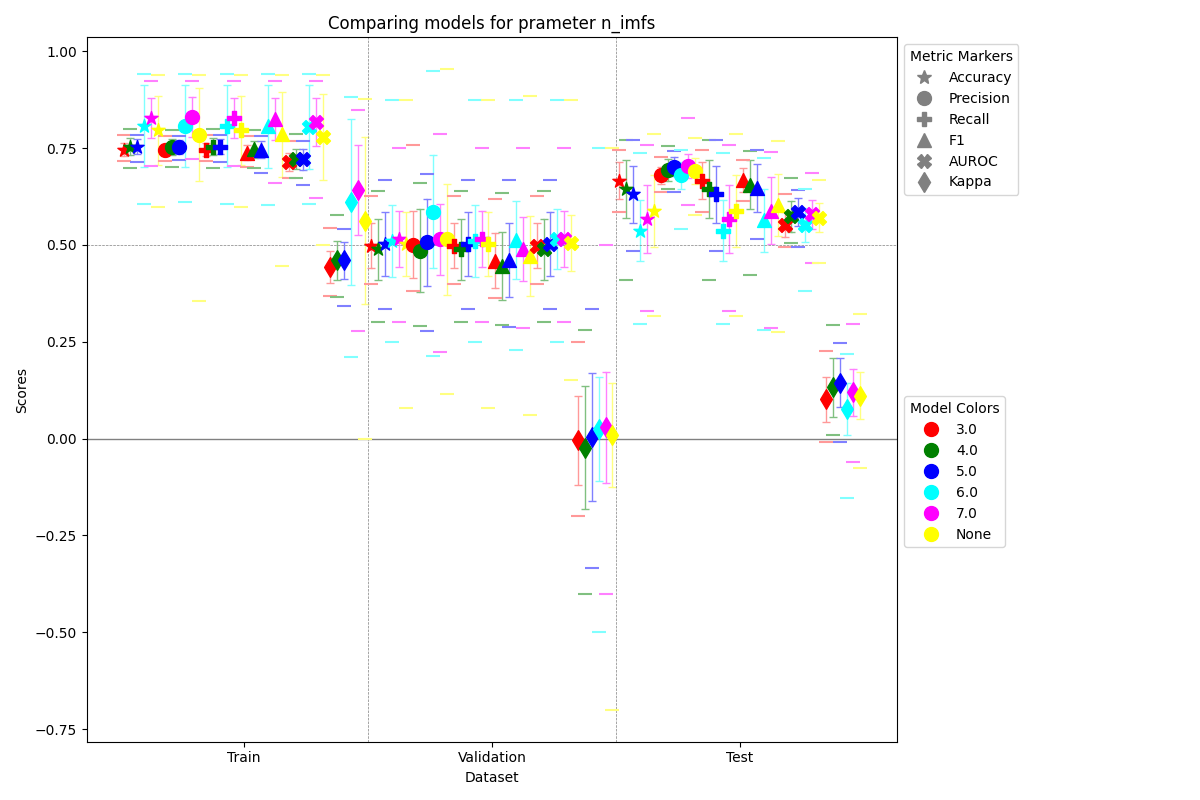
\includegraphics[width=400px]{Figures/results/n_imfs/n_imfs.png}
    \caption{All models compared by the IMF Cleaning parameter, a none value signifies no cleaning (raw signal) while a number means the number of IMFs kept in the cleaned signal after sorting for importance.}
    \label{fig: n_imfs}
\end{figure}


In \autoref{fig: memd_data_augmentation_on_test_auroc}, the IMF Cleaning parameters are plotted for the models scoring the best on the Test set metric AUROC. This means that there are only six different models plotted. It's clear that not cleaning scores worse on all sets. All the models seem to score more closely on the test set, with more significant discrepancies on the other sets. 


\begin{figure}[H]
    \centering
    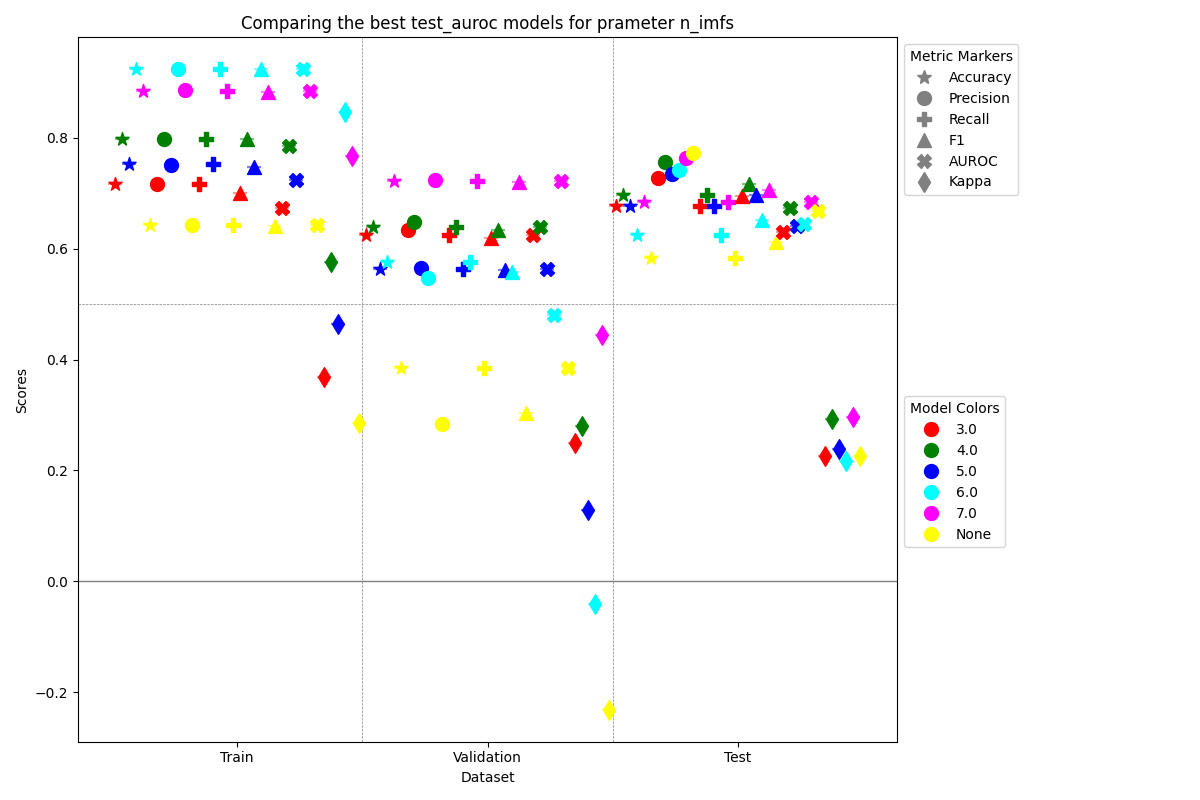
\includegraphics[width=400px]{Figures/results/n_imfs/n_imfs_test_auroc.png}
    \caption{The best models selected on the Test set AUROC score compared by the IMF Cleaning parameter.}
    \label{fig: n_imfs_test_auroc}
\end{figure}

\begin{comment}

\begin{figure}[H]
    \centering
    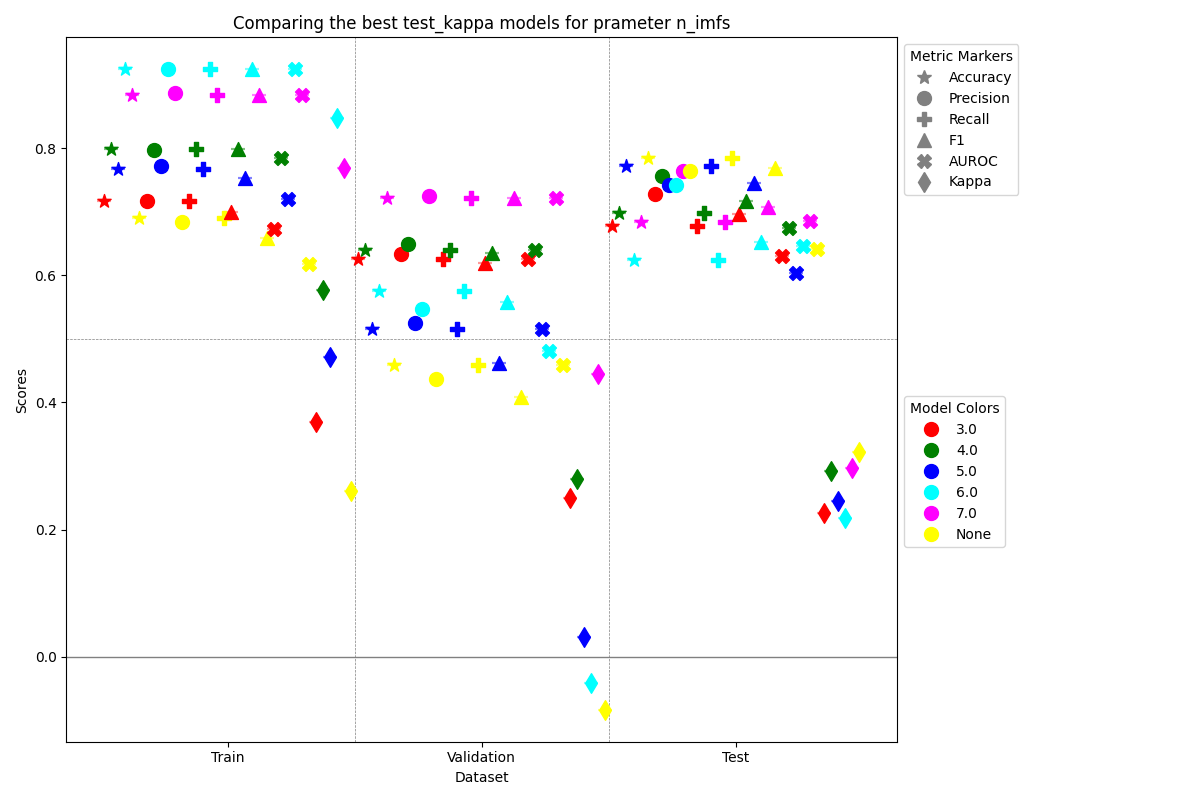
\includegraphics[width=400px]{Figures/results/n_imfs/n_imfs_test_kappa.png}
    \caption{The best models selected on the Test set Kappa score compared by the IMF cleaning parameter.}
    \label{fig: n_imfs_test_kappa}
\end{figure}

\begin{figure}[H]
    \centering
    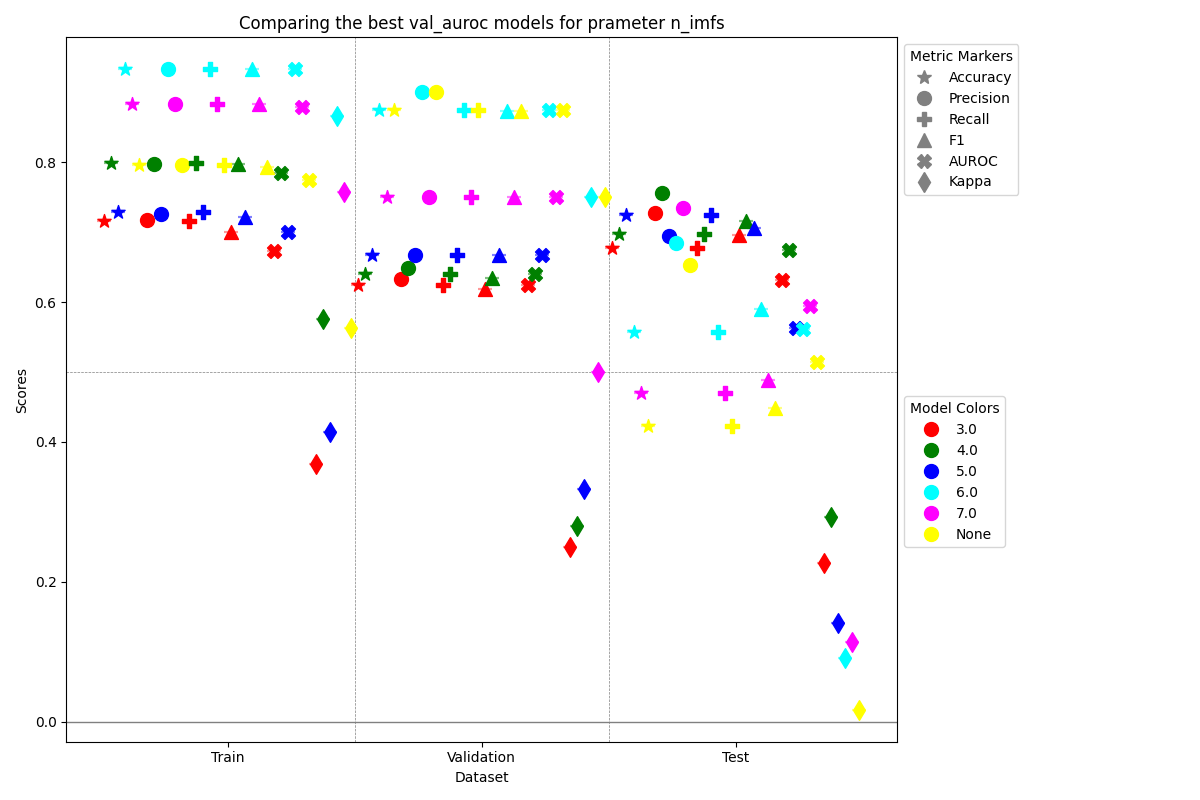
\includegraphics[width=400px]{Figures/results/n_imfs/n_imfs_val_auroc.png}
    \caption{The best models selected on the Validation set AUROC score compared by the IMF cleaning parameter.}
    \label{fig: n_imfs_val_auroc}
\end{figure}

\begin{figure}[H]
    \centering
    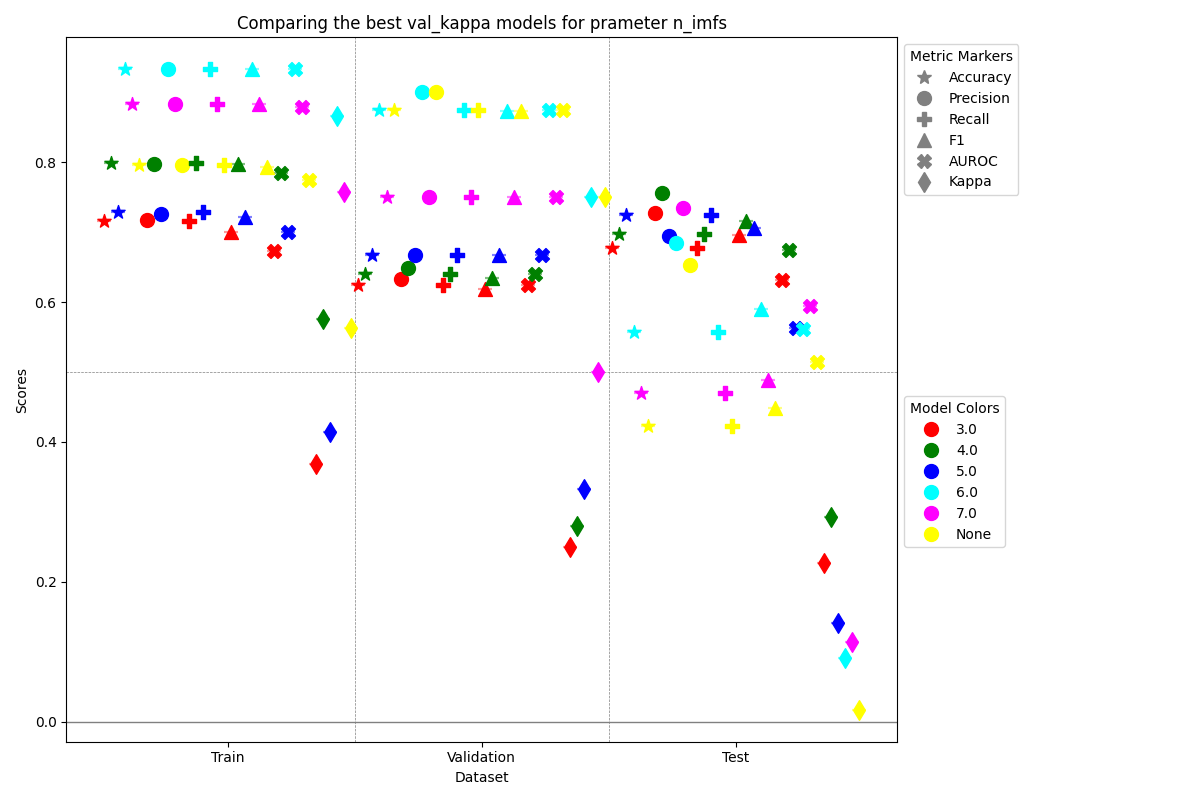
\includegraphics[width=400px]{Figures/results/n_imfs/n_imfs_val_kappa.png}
    \caption{The best models selected on the Validation set Kappa score compared by the IMF cleaning parameter.}
    \label{fig: n_imfs_val_kappa}
\end{figure}

\end{comment}


\section{Early Stopping Patience}
The Early Stopping Patience parameter is an integer value indicating how often the model can score worse than its best score on the Validation set for longer before the training loop is terminated. This is done to prevent overfitting to the training data. A higher value means the model can worsen for more epochs, potentially escaping local minima. A lower value potentially secures less overfitting.

For similar reasons as in \autoref{res_sec: memd_ratio}, only the statistics plot and the models scoring the best on the Test set using the metric Kappa will be displayed in the results. 

In \autoref{fig: patience}, the difference statistics between different Early Stopping Patience parameter values are compared on the three sets. Similarly to \autoref{res_sec: memd_ratio}, it is hard to see the individual values due to the number of metrics and parameter values plotted. However, this is chosen to showcase trends rather than personal values. It's clear from the Training set that higher Patience causes better results on all metrics. This does not seem to transfer to the other sets, where the relationship is less evident in both the average and extreme cases.


\begin{figure}[H]
    \centering
    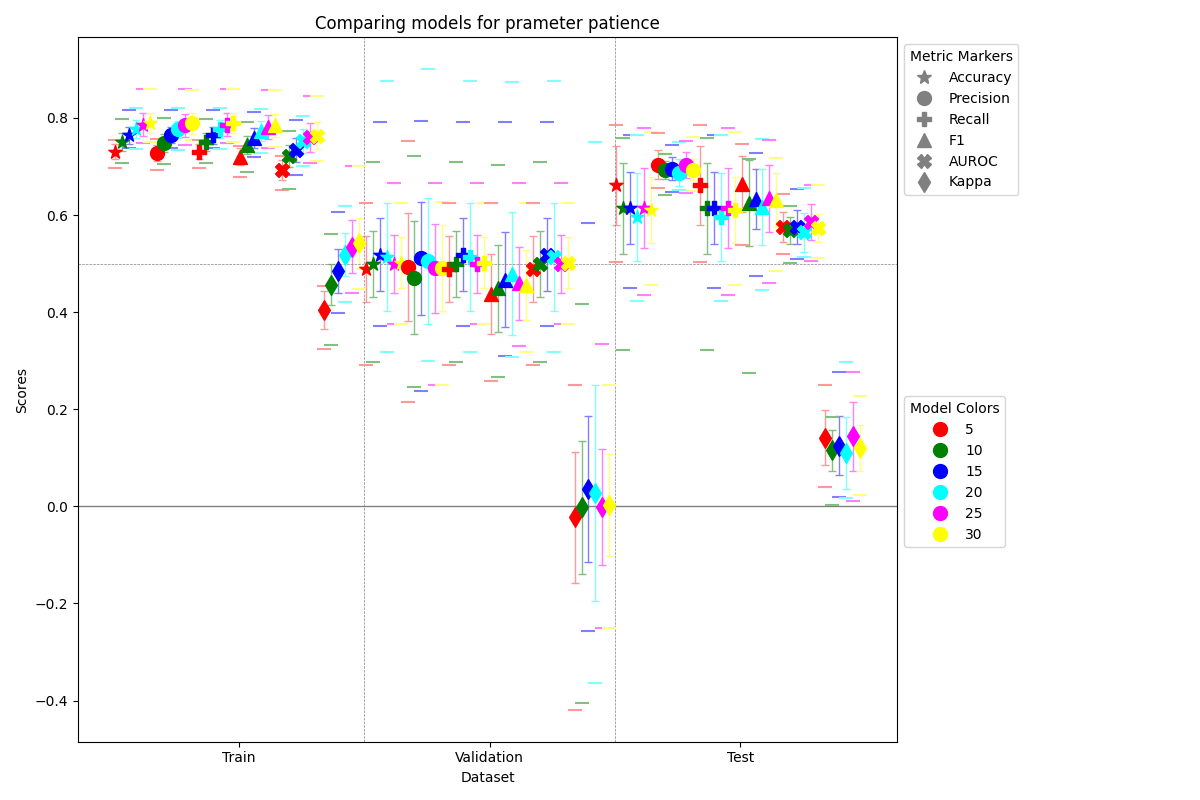
\includegraphics[width=400px]{Figures/results/patience/patience.png}
    \caption{All models compared by the Early Stopping Patience parameter, a higher value means the model can score worse than the best score on the Validation set so far for longer before the training loop is terminated.}
    \label{fig: patience}
\end{figure}


In \autoref{fig: patience_test_kappa}, the Early Stopping Patience parameters are plotted for the models scoring the best on the Test set metric Kappa. This means that there are only six different models plotted. Just like in the statistics case, it is clear from the Training set that higher Patience causes better results on all metrics. This does not seem to transfer well to the other sets. In the Test set, the relationship is weaker, but the parameter values from 15 to 25 seem to have the highest scores.

\begin{figure}[H]
    \centering
    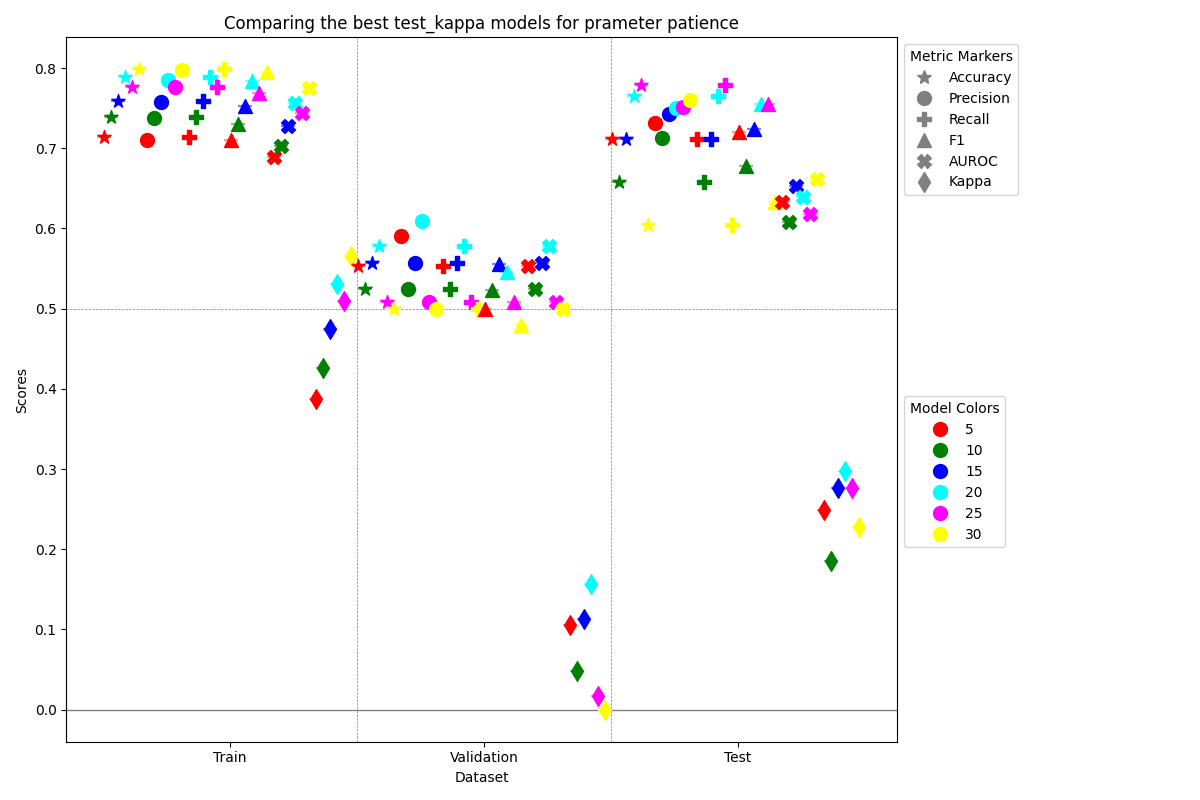
\includegraphics[width=400px]{Figures/results/patience/patience_test_kappa.png}
    \caption{The best models selected on the Test set Kappa score compared by the Early Stopping Patience parameter.}
    \label{fig: patience_test_kappa}
\end{figure}

\begin{comment}


\begin{figure}[H]
    \centering
    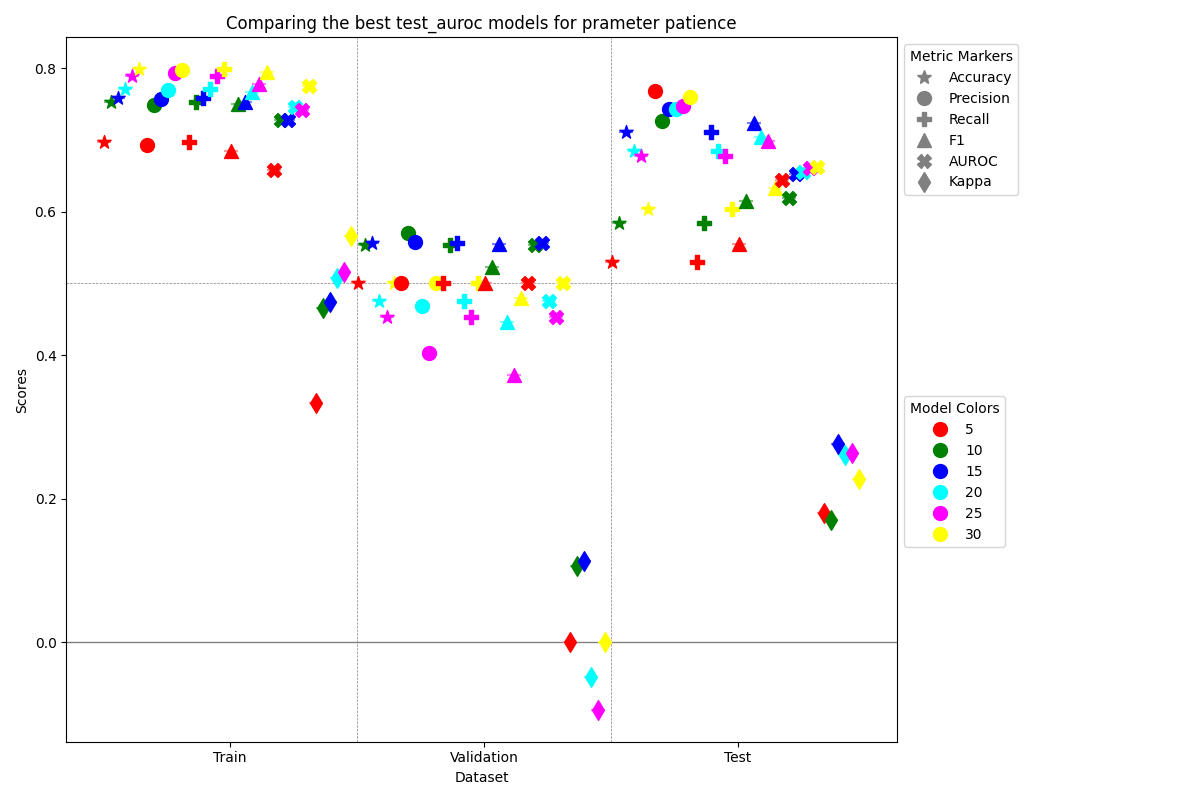
\includegraphics[width=400px]{Figures/results/patience/patience_test_auroc.png}
    \caption{The best models selected on the Test set AUROC score compared by the Early Stopping Patience parameter.}
    \label{fig: patience_test_auroc}
\end{figure}


\begin{figure}[H]
    \centering
    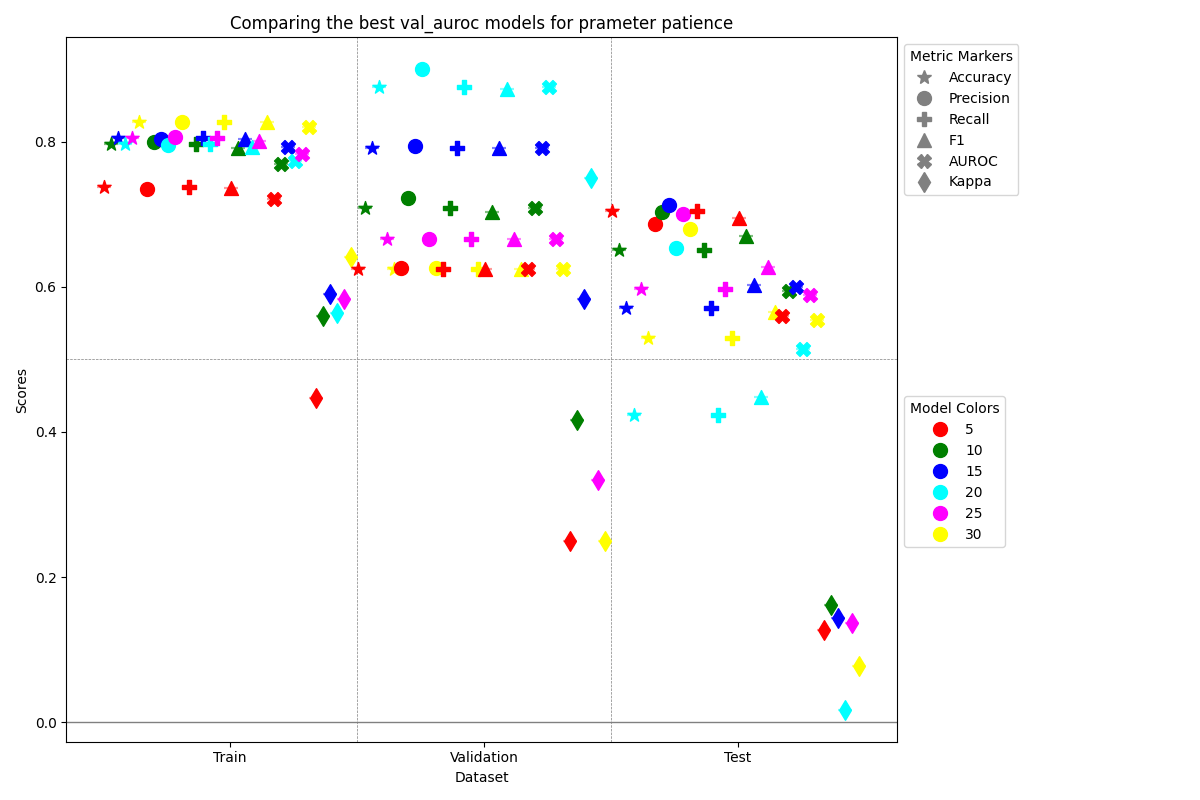
\includegraphics[width=400px]{Figures/results/patience/patience_val_auroc.png}
    \caption{The best models selected on the Validation set AUROC score compared by the Early Stopping Patience parameter.}
    \label{fig: patience_val_auroc}
\end{figure}

\begin{figure}[H]
    \centering
    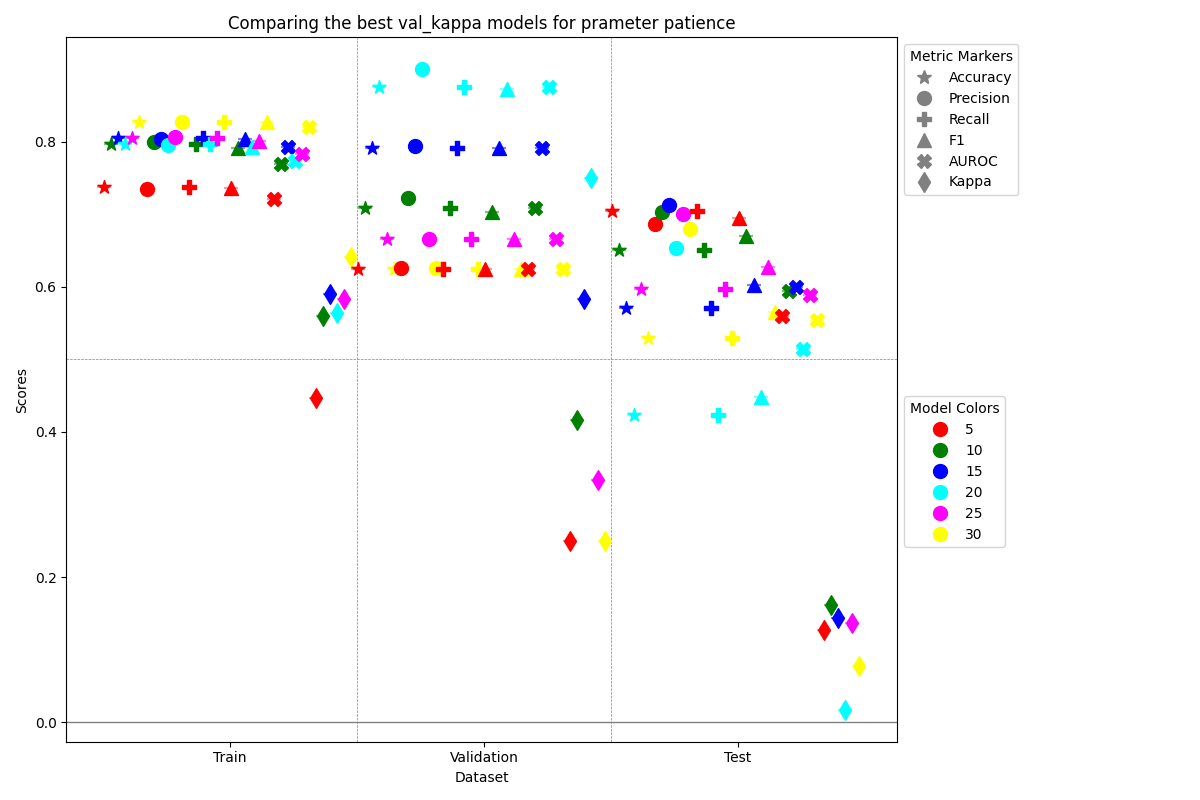
\includegraphics[width=400px]{Figures/results/patience/patience_val_kappa.png}
    \caption{The best models selected on the Validation set Kappa score compared by the Early Stopping Patience parameter.}
    \label{fig: patience_val_kappa}
\end{figure}

\end{comment}


\section{Regularization Techniques}
The Regularization Technique parameter is a string or None value parameter. The None value means no regularization is done on the data, while the string values of l1 or l2 choose the regularization method to regularize the data. The different techniques are explained in \autoref{subsec: regularization}.

In \autoref{fig: reg_type}, the difference statistics between different Regularization Technique parameter values are compared on the three sets. The L1 parameter value scores are lower or equal on all metrics and all average case sets. Looking at the maximum values, L1 also scores lower on most metrics. L2 and no regularization scores are very similar in the average case on all metrics, but in the extreme case, L2 scores are better for most metrics.

\begin{figure}[H]
    \centering
    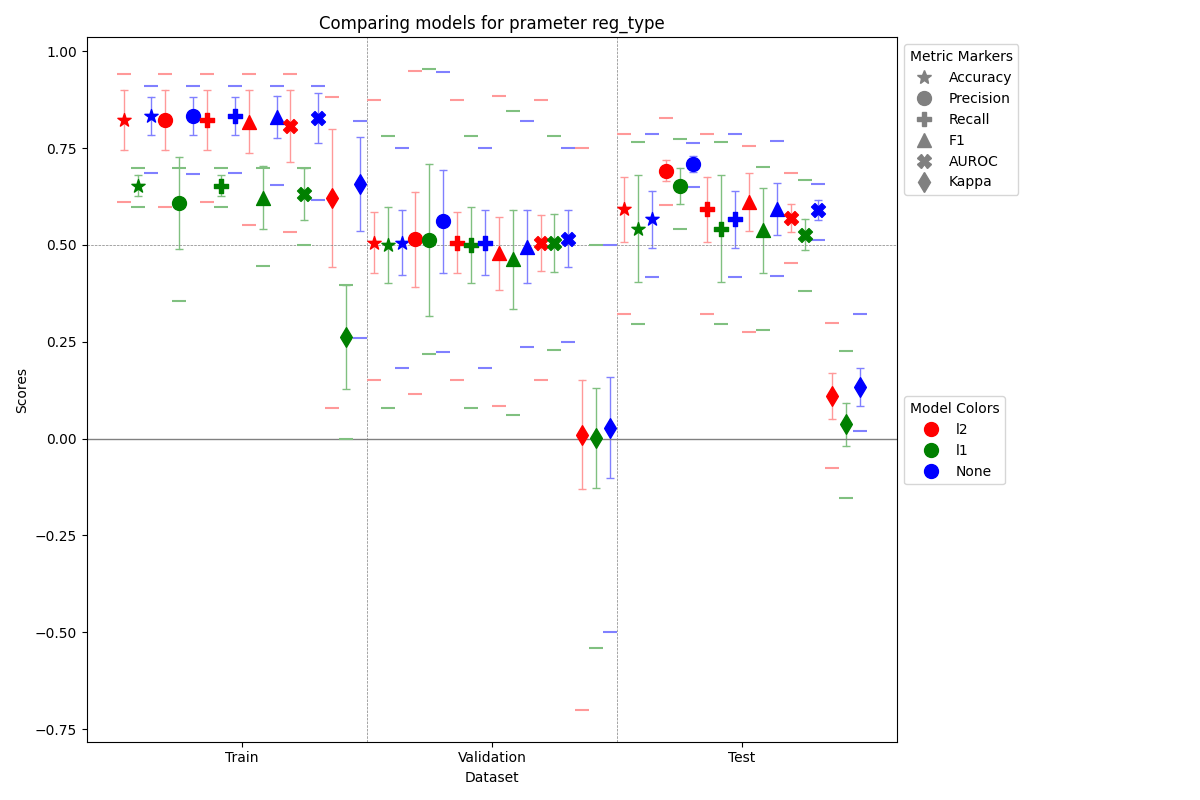
\includegraphics[width=400px]{Figures/results/reg_type/reg_type.png}
    \caption{All models compared by the Regularization Techniques parameter, the different methods are explained in \autoref{subsec: regularization}.}
    \label{fig: reg_type}
\end{figure}

In \autoref{fig: reg_type_test_auroc}, the Regularization Technique parameters are plotted for the models scoring the best on the Test set metric AUROC. This means that there are only three different models plotted. Just like in the statistics case, it is clear that L1 scores lower on most metrics. L2 has a good correspondence between sets, with the model scoring similarly on the Validation and Test sets. The no-regularization model varies from set to set and gets the best results for the test set.

\begin{figure}[H]
    \centering
    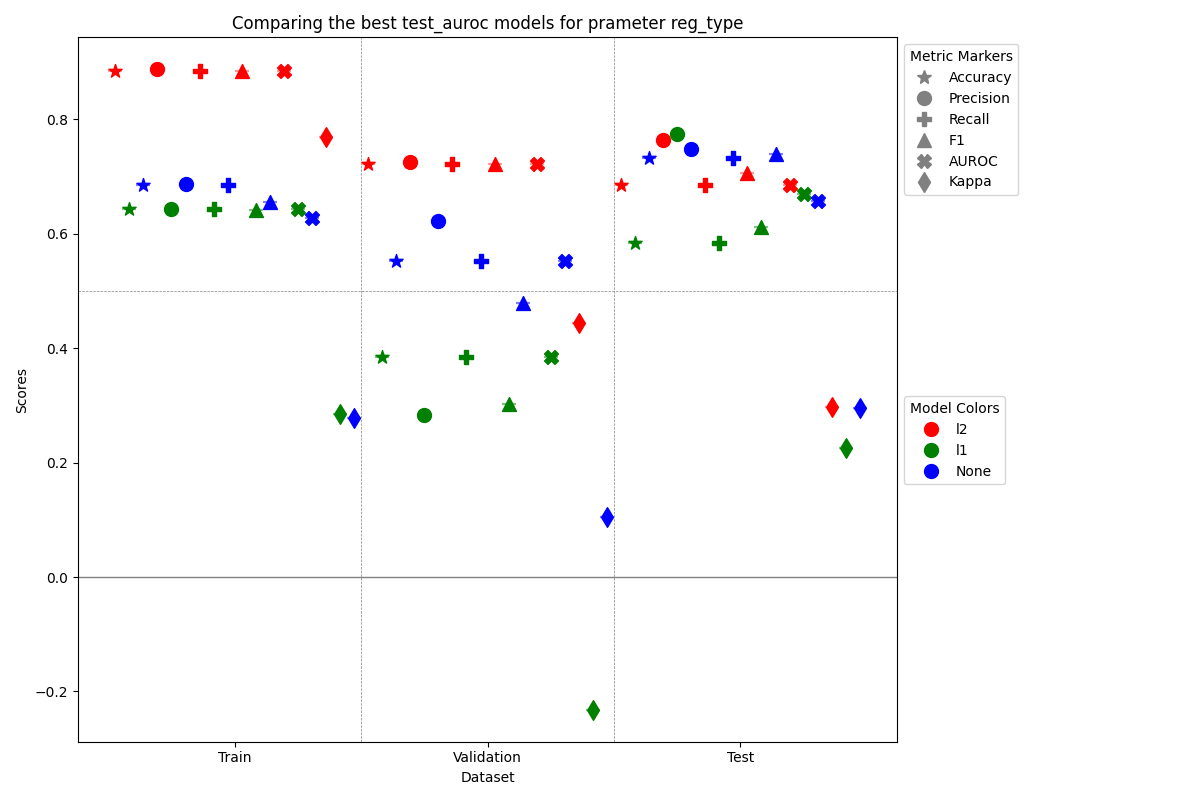
\includegraphics[width=400px]{Figures/results/reg_type/reg_type_test_auroc.png}
    \caption{The best models selected on the Test set AUROC score compared by the Regularization Techniques parameter.}
    \label{fig: reg_type_test_auroc}
\end{figure}

\begin{comment}

\begin{figure}[H]
    \centering
    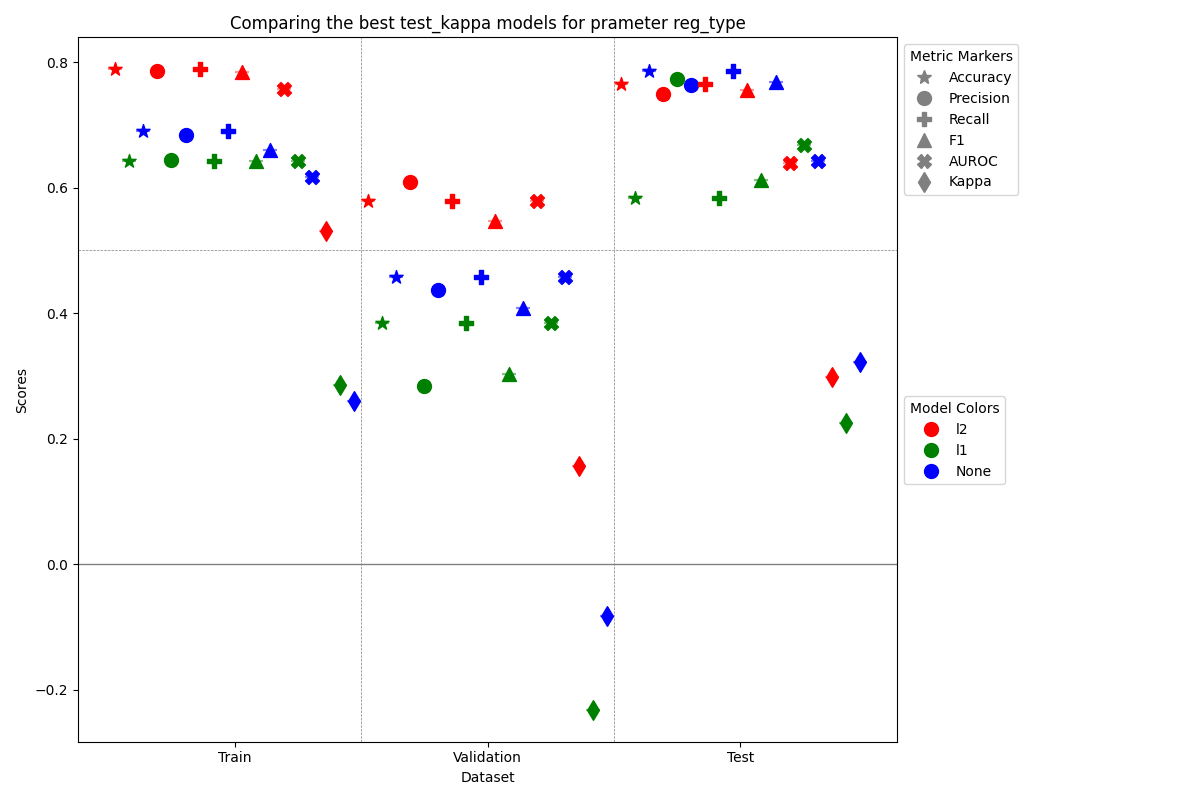
\includegraphics[width=400px]{Figures/results/reg_type/reg_type_test_kappa.png}
    \caption{The best models selected on the Test set Kappa score compared by the Regularization Techniques parameter.}
    \label{fig: reg_type_test_kappa}
\end{figure}

\begin{figure}[H]
    \centering
    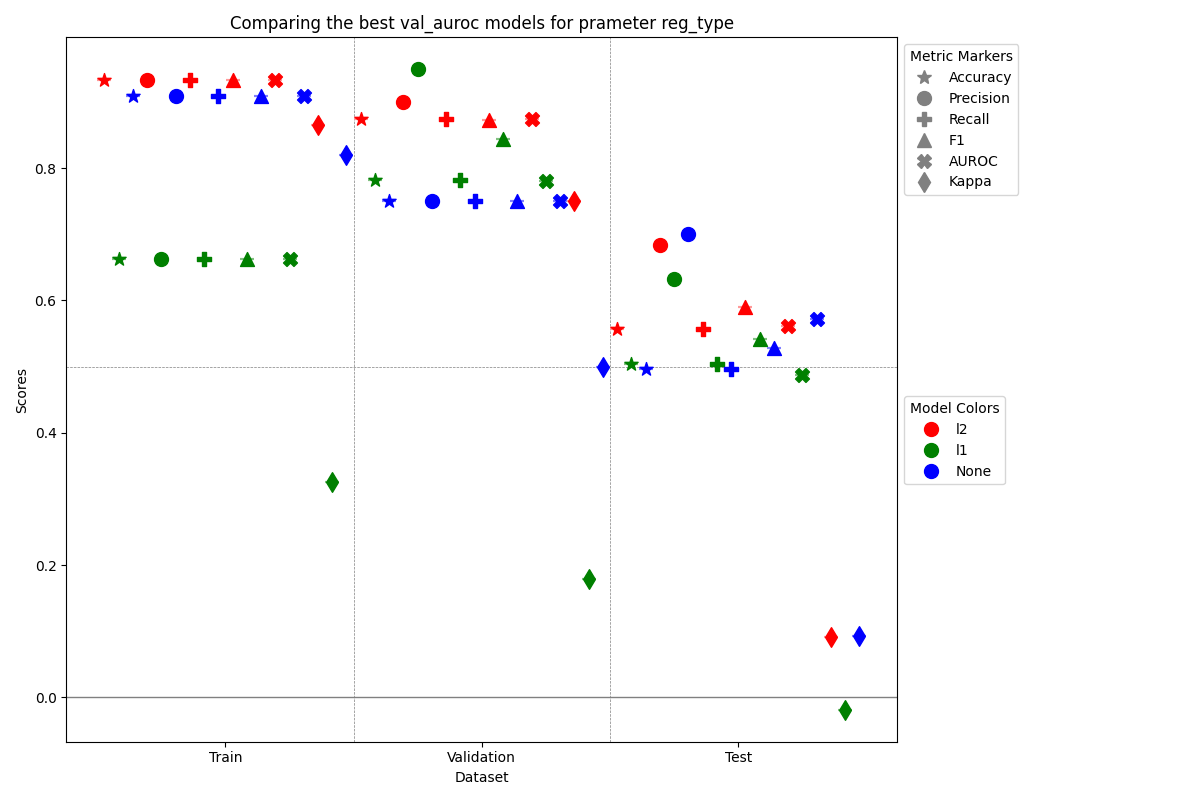
\includegraphics[width=400px]{Figures/results/reg_type/reg_type_val_auroc.png}
    \caption{The best models selected on the Validation set AUROC score compared by the Regularization Techniques parameter.}
    \label{fig: reg_type_val_auroc}
\end{figure}

\begin{figure}[H]
    \centering
    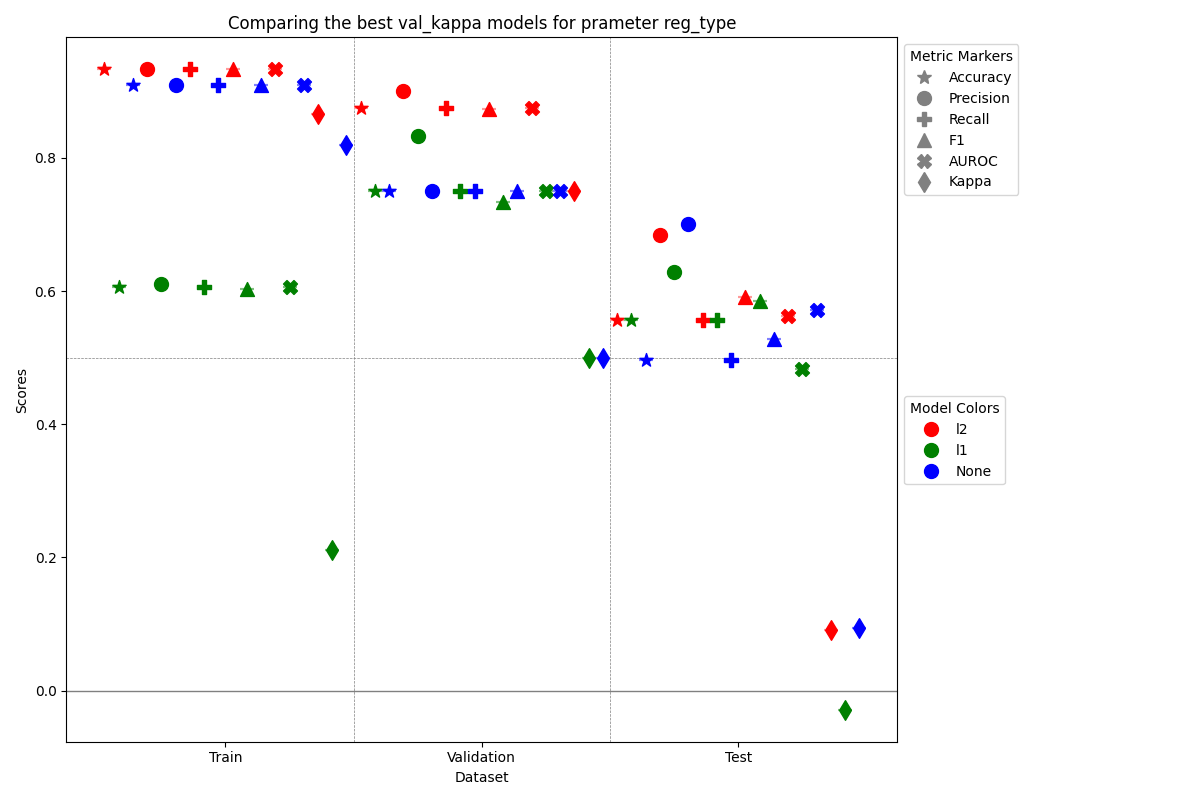
\includegraphics[width=400px]{Figures/results/reg_type/reg_type_val_kappa.png}
    \caption{The best models selected on the Validation set Kappa score compared by the Regularization Techniques parameter.}
    \label{fig: reg_type_val_kappa}
\end{figure}

\end{comment}






\section{Regularization Value}
This section compares different regularization values for the L2 method. A higher value means larger node values are punished harder, as explained in \autoref{subsec: regularization}. This tends to drive down the score on the training set as it overfits the training data less.

In \autoref{fig: reg_val}, the statistics of the difference between different Regularization Value parameter values are compared on the three sets. As expected, the scores on the Training set are inversely proportional to the Regularization Value. The average scores on the other sets are similar for all metrics, while the values of 0.05 and 0.1 score better in the extreme on both the Test and Validation sets.

\begin{figure}[H]
    \centering
    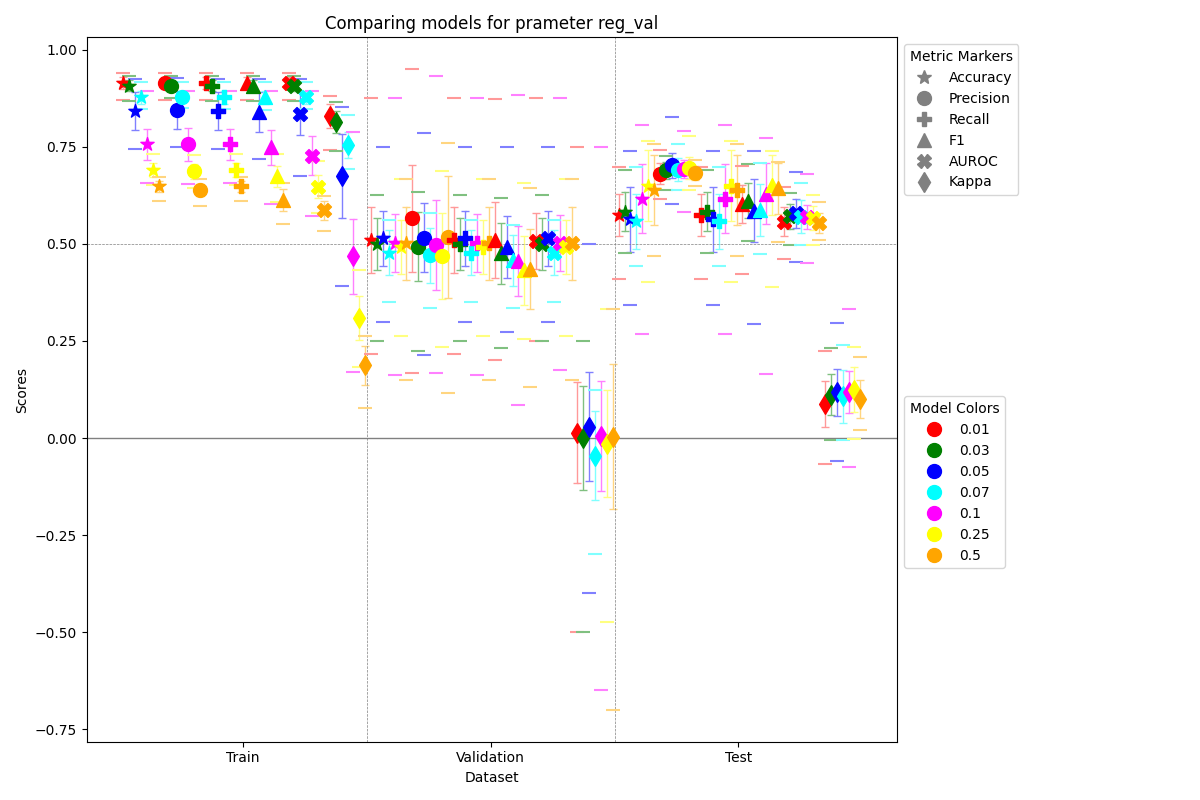
\includegraphics[width=400px]{Figures/results/reg_val/reg_val.png}
    \caption{All models compared by the Regularization Value parameter for the L2 method, a higher value means more regularization.}
    \label{fig: reg_val}
\end{figure}

In \autoref{fig: reg_val_test_auroc}, the Regularization Value parameters are plotted for the models scoring the best on the Test set metric AUROC. This means that there are only seven different models plotted. Just like in the statistics case, the scores on the training set align well with expectations. The 0.1 value scores best on most metrics in the Test set, while the 0.05 value has the best correspondence between the three sets while getting good scores.

\begin{figure}[H]
    \centering
    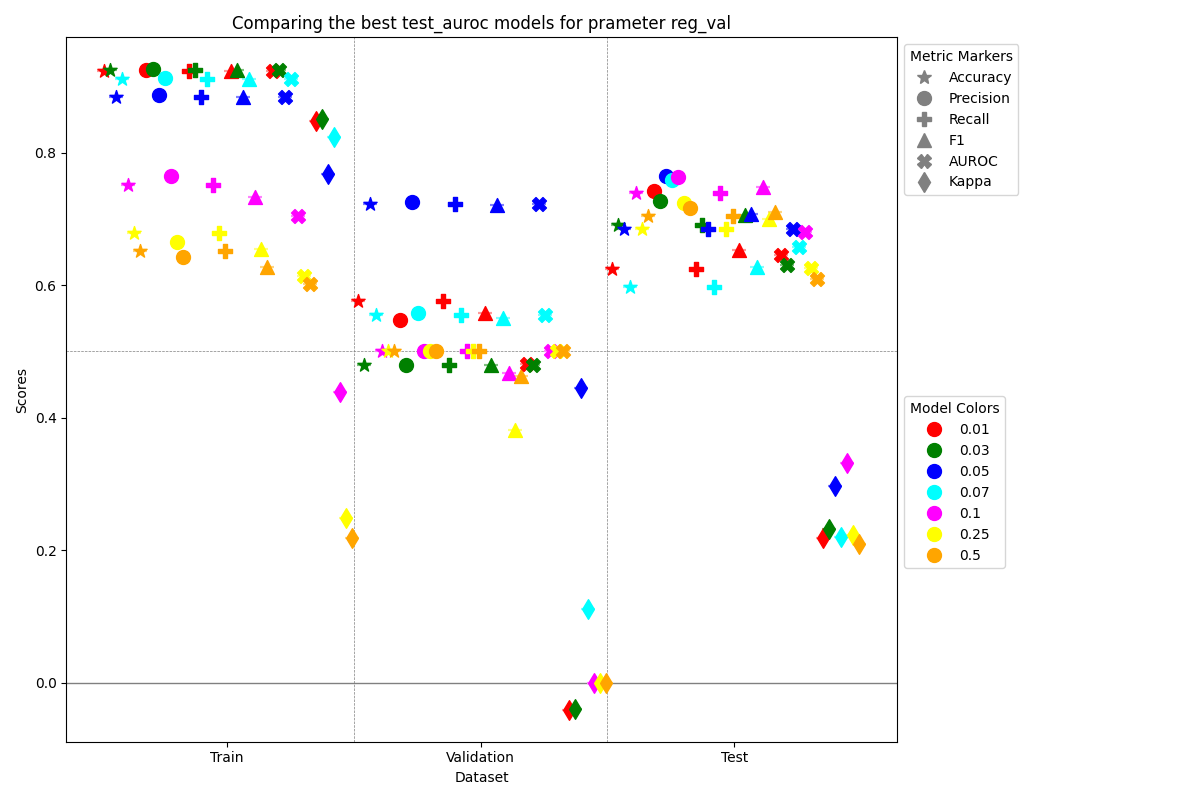
\includegraphics[width=400px]{Figures/results/reg_val/reg_val_test_auroc.png}
    \caption{The best models selected on the Test set AUROC score compared by the Regularization Value parameter.}
    \label{fig: reg_val_test_auroc}
\end{figure}


\begin{comment}

\begin{figure}[H]
    \centering
    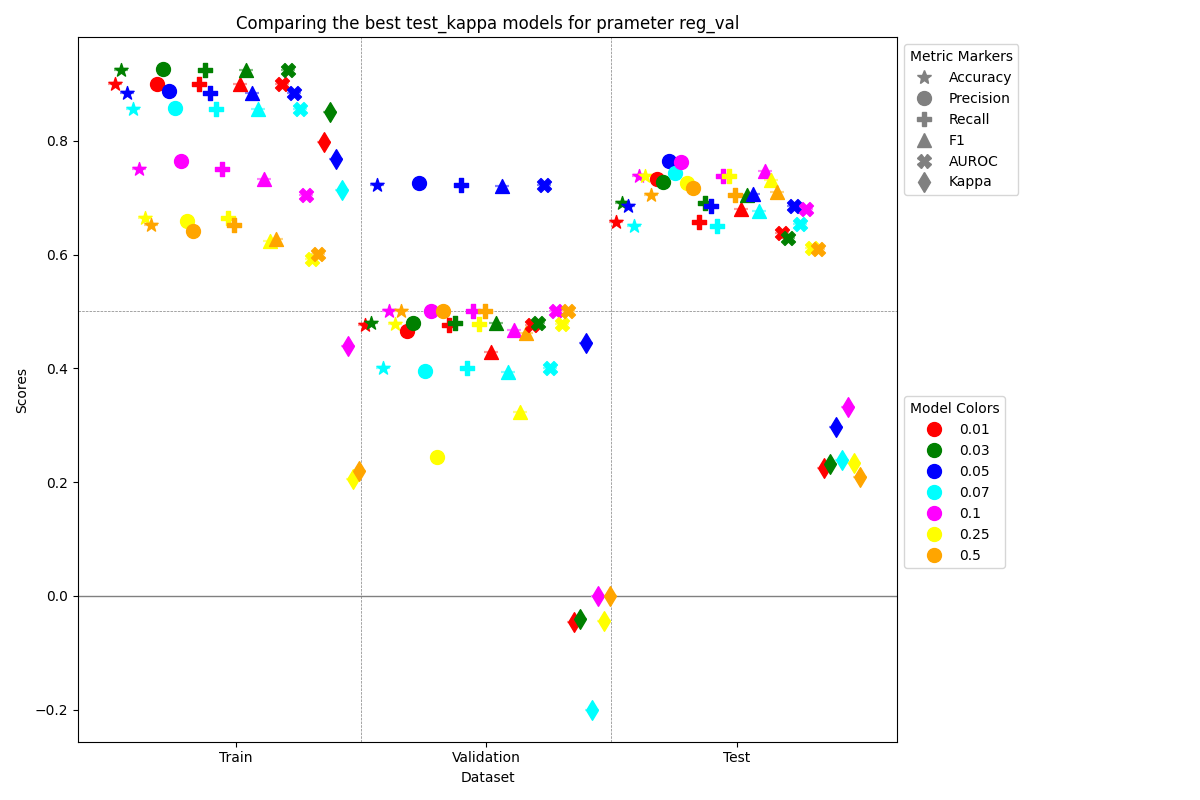
\includegraphics[width=400px]{Figures/results/reg_val/reg_val_test_kappa.png}
    \caption{The best models selected on the Test set Kappa score compared by the Regularization Value parameter.}
    \label{fig: reg_val_test_kappa}
\end{figure}

\begin{figure}[H]
    \centering
    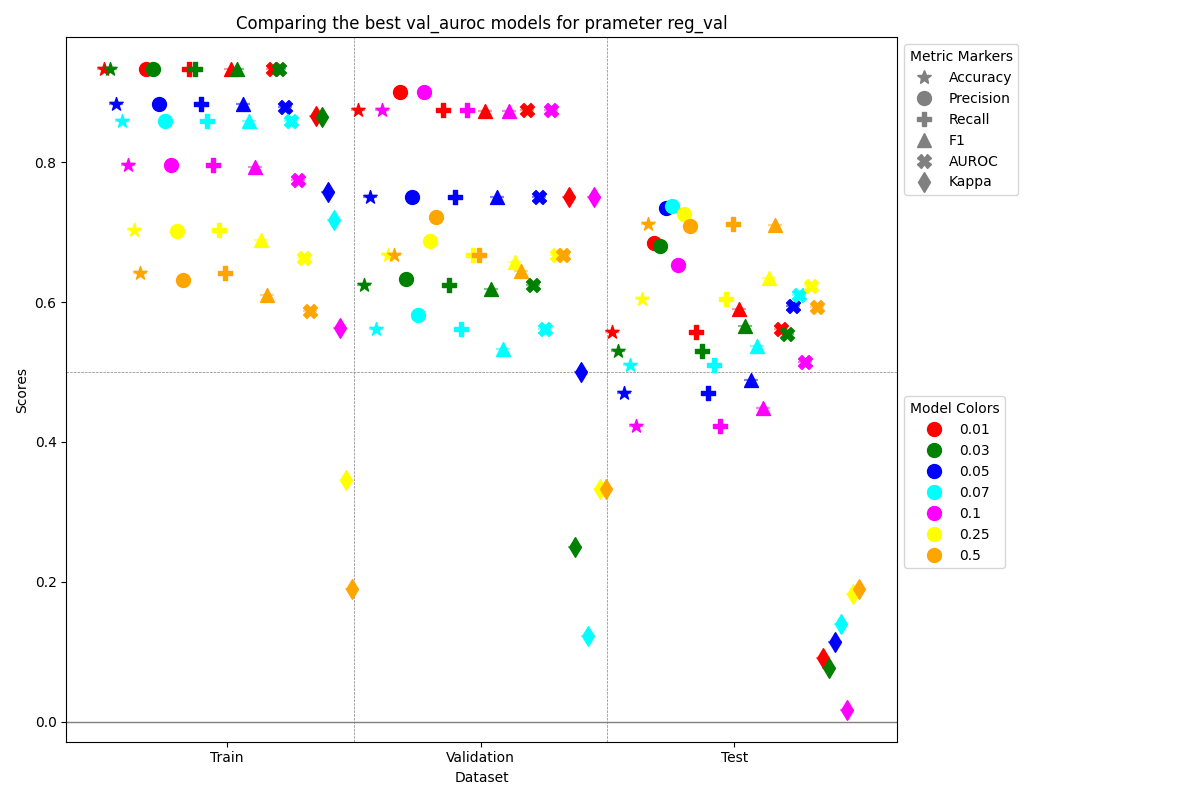
\includegraphics[width=400px]{Figures/results/reg_val/reg_val_val_auroc.png}
    \caption{The best models selected on the Validation set AUROC score compared by the Regularization Value parameter.}
    \label{fig: reg_val_val_auroc}
\end{figure}

\begin{figure}[H]
    \centering
    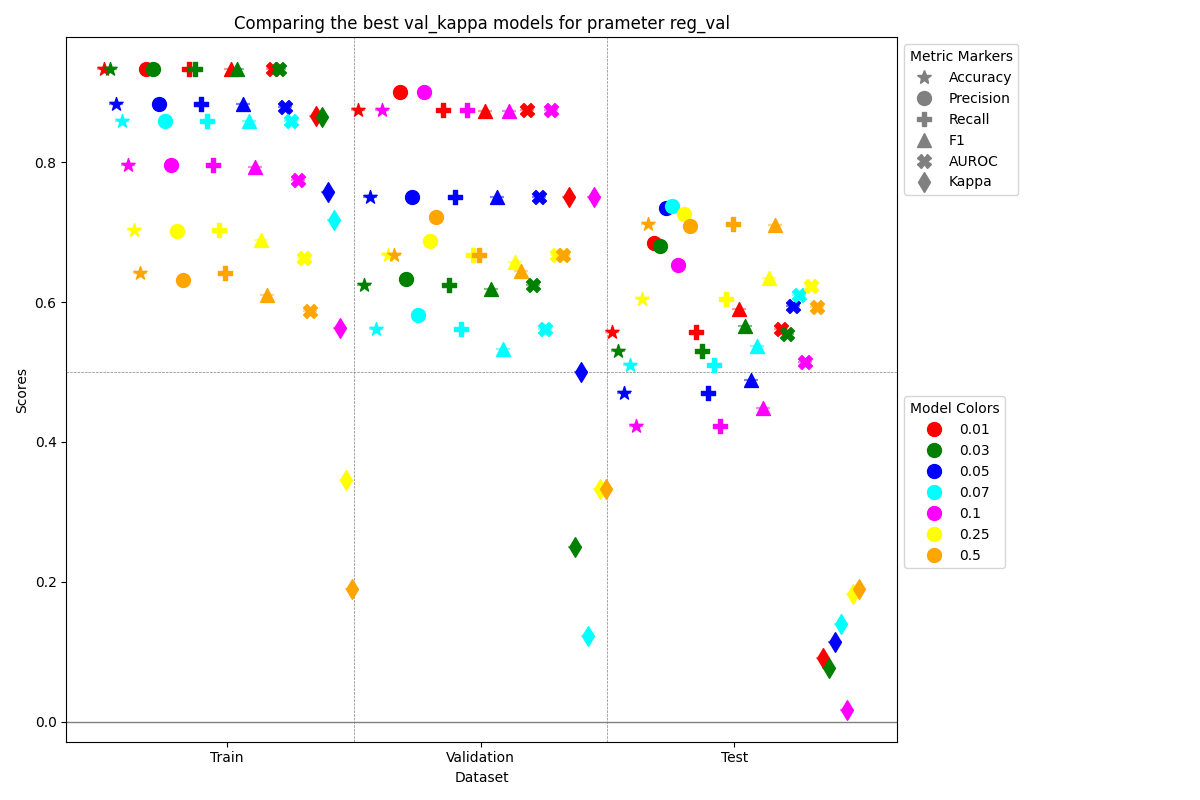
\includegraphics[width=400px]{Figures/results/reg_val/reg_val_val_kappa.png}
    \caption{The best models selected on the Validation set Kappa score compared by the Regularization Value parameter.}
    \label{fig: reg_val_val_kappa}
\end{figure}

\end{comment}


\section{Dropout Rate}
This section compares different dropout rate values. A higher Dropout Rate means more network nodes are turned off at offndom during training as explained in \autoref{subsec: regularization}. This tends to drive down the score on the training set as it overfits the training data less.

In \autoref{fig: dropout}, the difference statistics between different Dropout Rate parameter values are compared in \ three sets. As expected, the scores on the Training set are inversely proportional to the Dropout Rate. The average scores on the Test set seem to be proportional to the Dropout Rate value, while on the Validation set, most values score similarly. 

\begin{figure}[H]
    \centering
    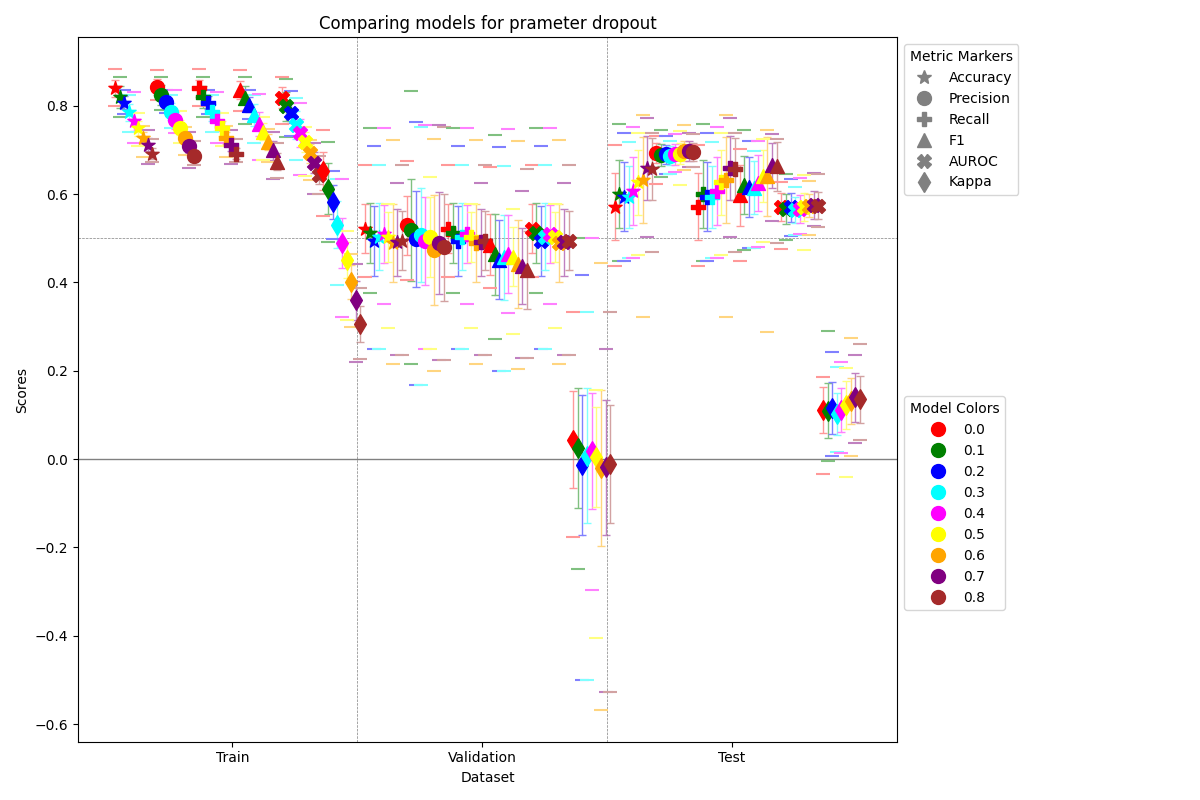
\includegraphics[width=400px]{Figures/results/dropout/dropout.png}
    \caption{All models compared by the Dropout Rate parameter, a higher value means more dropout.}
    \label{fig: dropout}
\end{figure}

In \autoref{fig: dropout_test_auroc}, the Dropout Rate parameters are plotted for the models scoring the best on the Test set metric AUROC. This means that there are only nine different models plotted. Just like in the statistics case, the scores on the training set align well with expectations. The values 0.1 and 0.6 seem to score the highest on most metrics in the Test set, while 0.8 seems to have the most correspondence between scores across the different sets.


\begin{figure}[H]
    \centering
    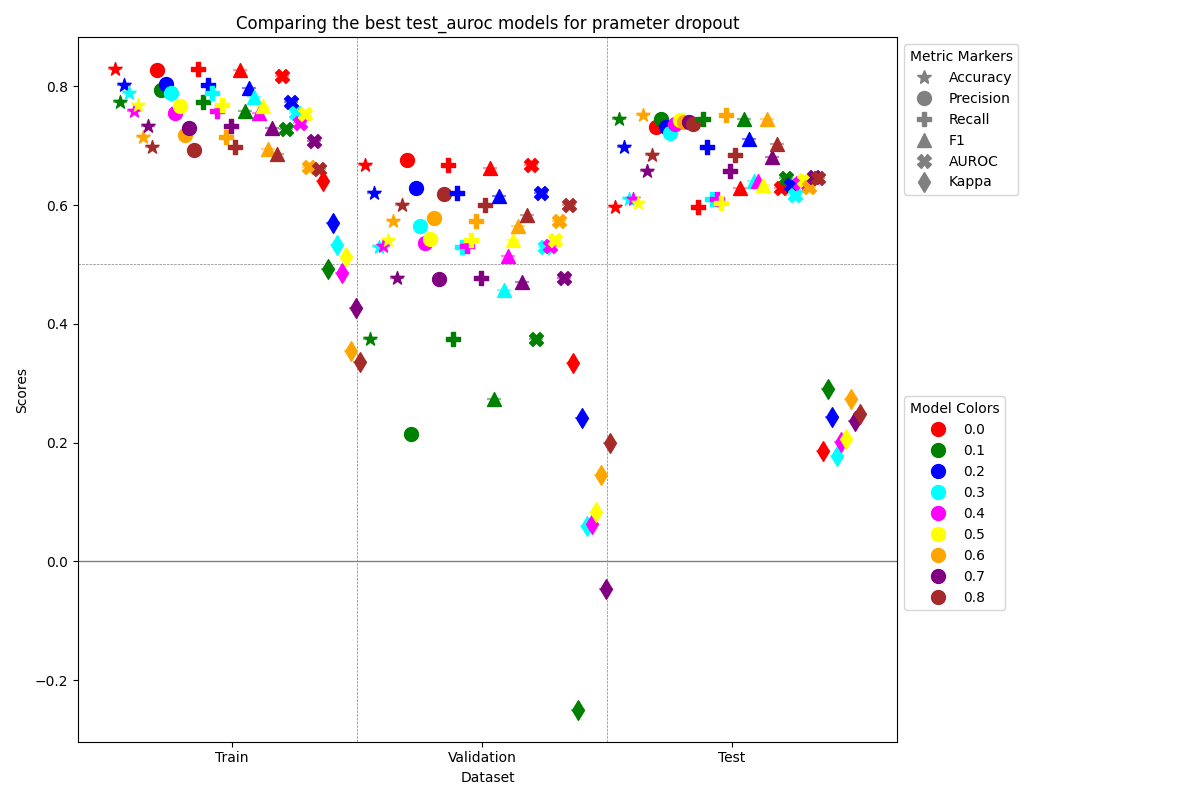
\includegraphics[width=400px]{Figures/results/dropout/dropout_test_auroc.png}
    \caption{The best models selected on the Test set AUROC score compared by the Dropout Rate parameter.}
    \label{fig: dropout_test_auroc}
\end{figure}
\begin{comment}
\begin{figure}[H]
    \centering
    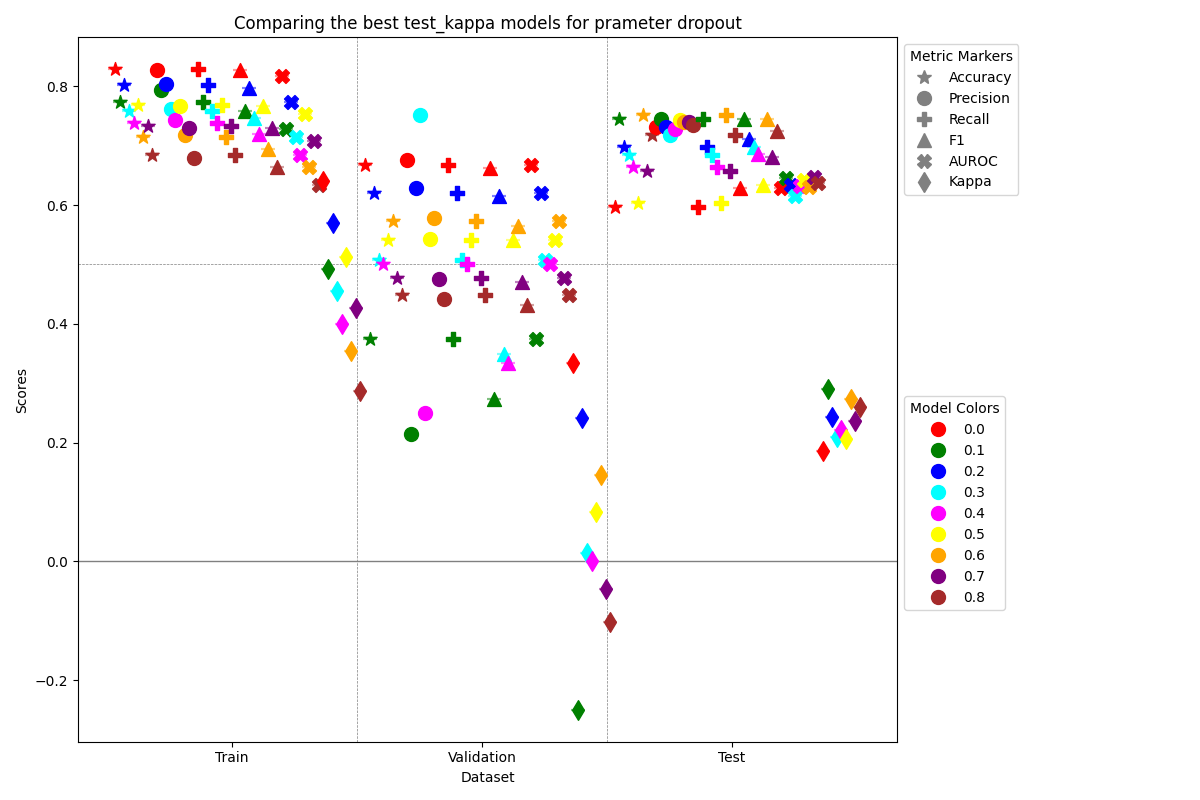
\includegraphics[width=400px]{Figures/results/dropout/dropout_test_kappa.png}
    \caption{The best models selected on the Test set Kappa score compared by the Dropout Rate parameter.}
    \label{fig: dropout_test_kappa}
\end{figure}

\begin{figure}[H]
    \centering
    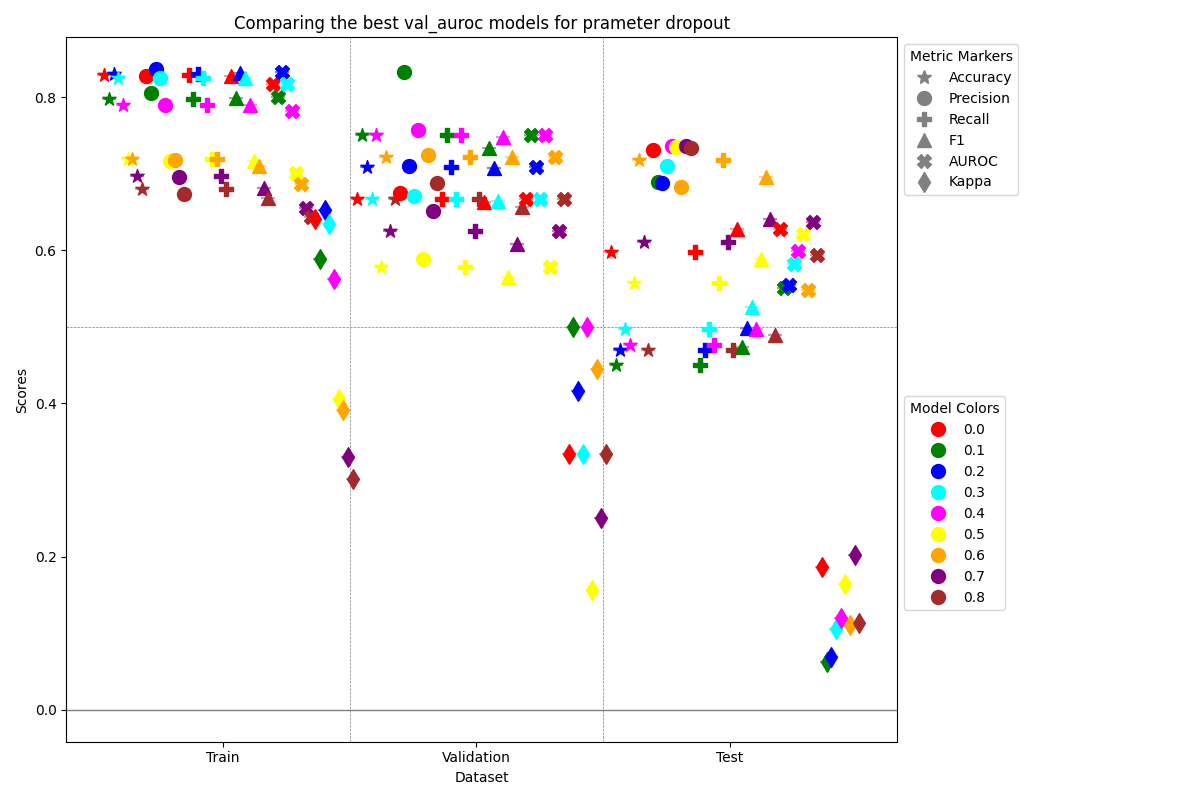
\includegraphics[width=400px]{Figures/results/dropout/dropout_val_auroc.png}
    \caption{The best models selected on the Validation set AUROC score compared by the Dropout Rate parameter.}
    \label{fig: dropout_val_auroc}
\end{figure}

\begin{figure}[H]
    \centering
    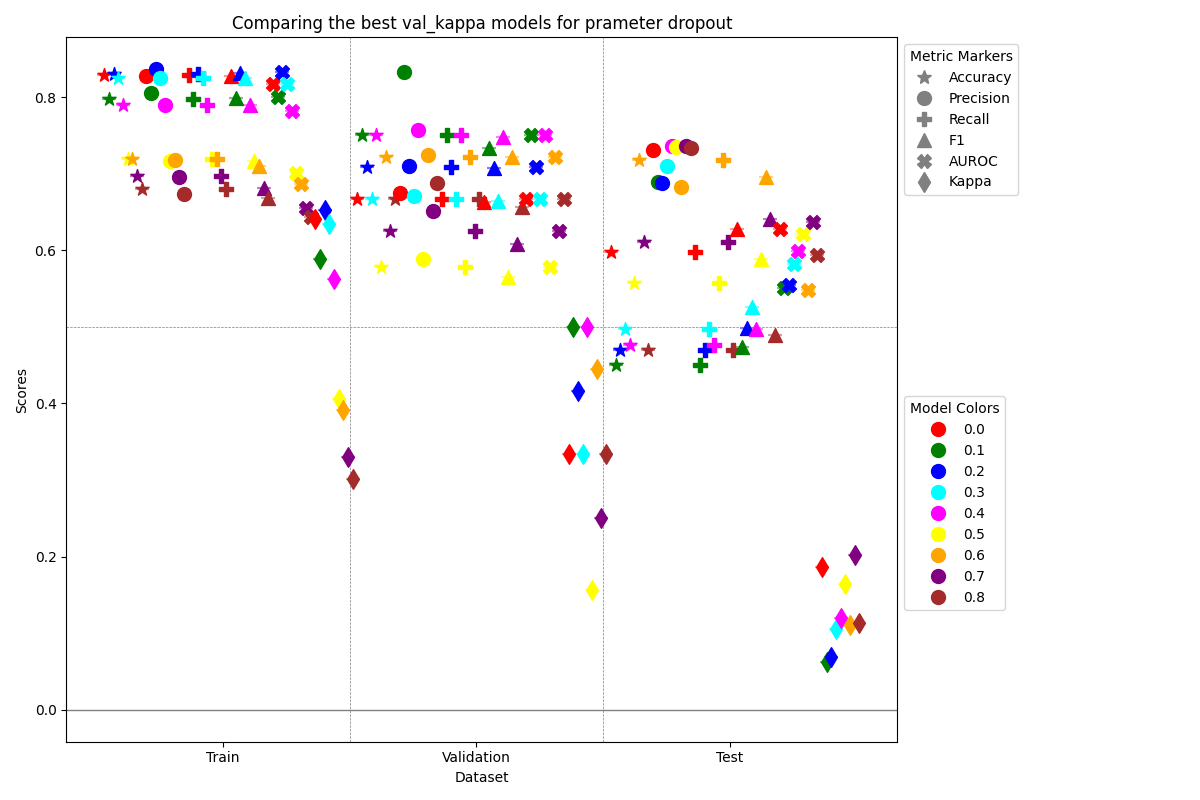
\includegraphics[width=400px]{Figures/results/dropout/dropout_val_kappa.png}
    \caption{The best models selected on the Validation set Kappa score compared by the Dropout Rate parameter.}
    \label{fig: dropout_val_kappa}
\end{figure}

\end{comment}

\section{Dataset}
The dataset distribution is plotted in \autoref{fig: dataset_dist}. The subject with the lowest amount of total epochs is Subject 1, with 107 epochs. The subject with the highest amount of total epochs is Subject 25, with 208. 2/3 subjects have more than twice as many of one epoch type than the other. Of these 20 subjects, 16 have more than twice as much OT, while four have more than twice as much MW.
\begin{figure}[H]
    \centering
    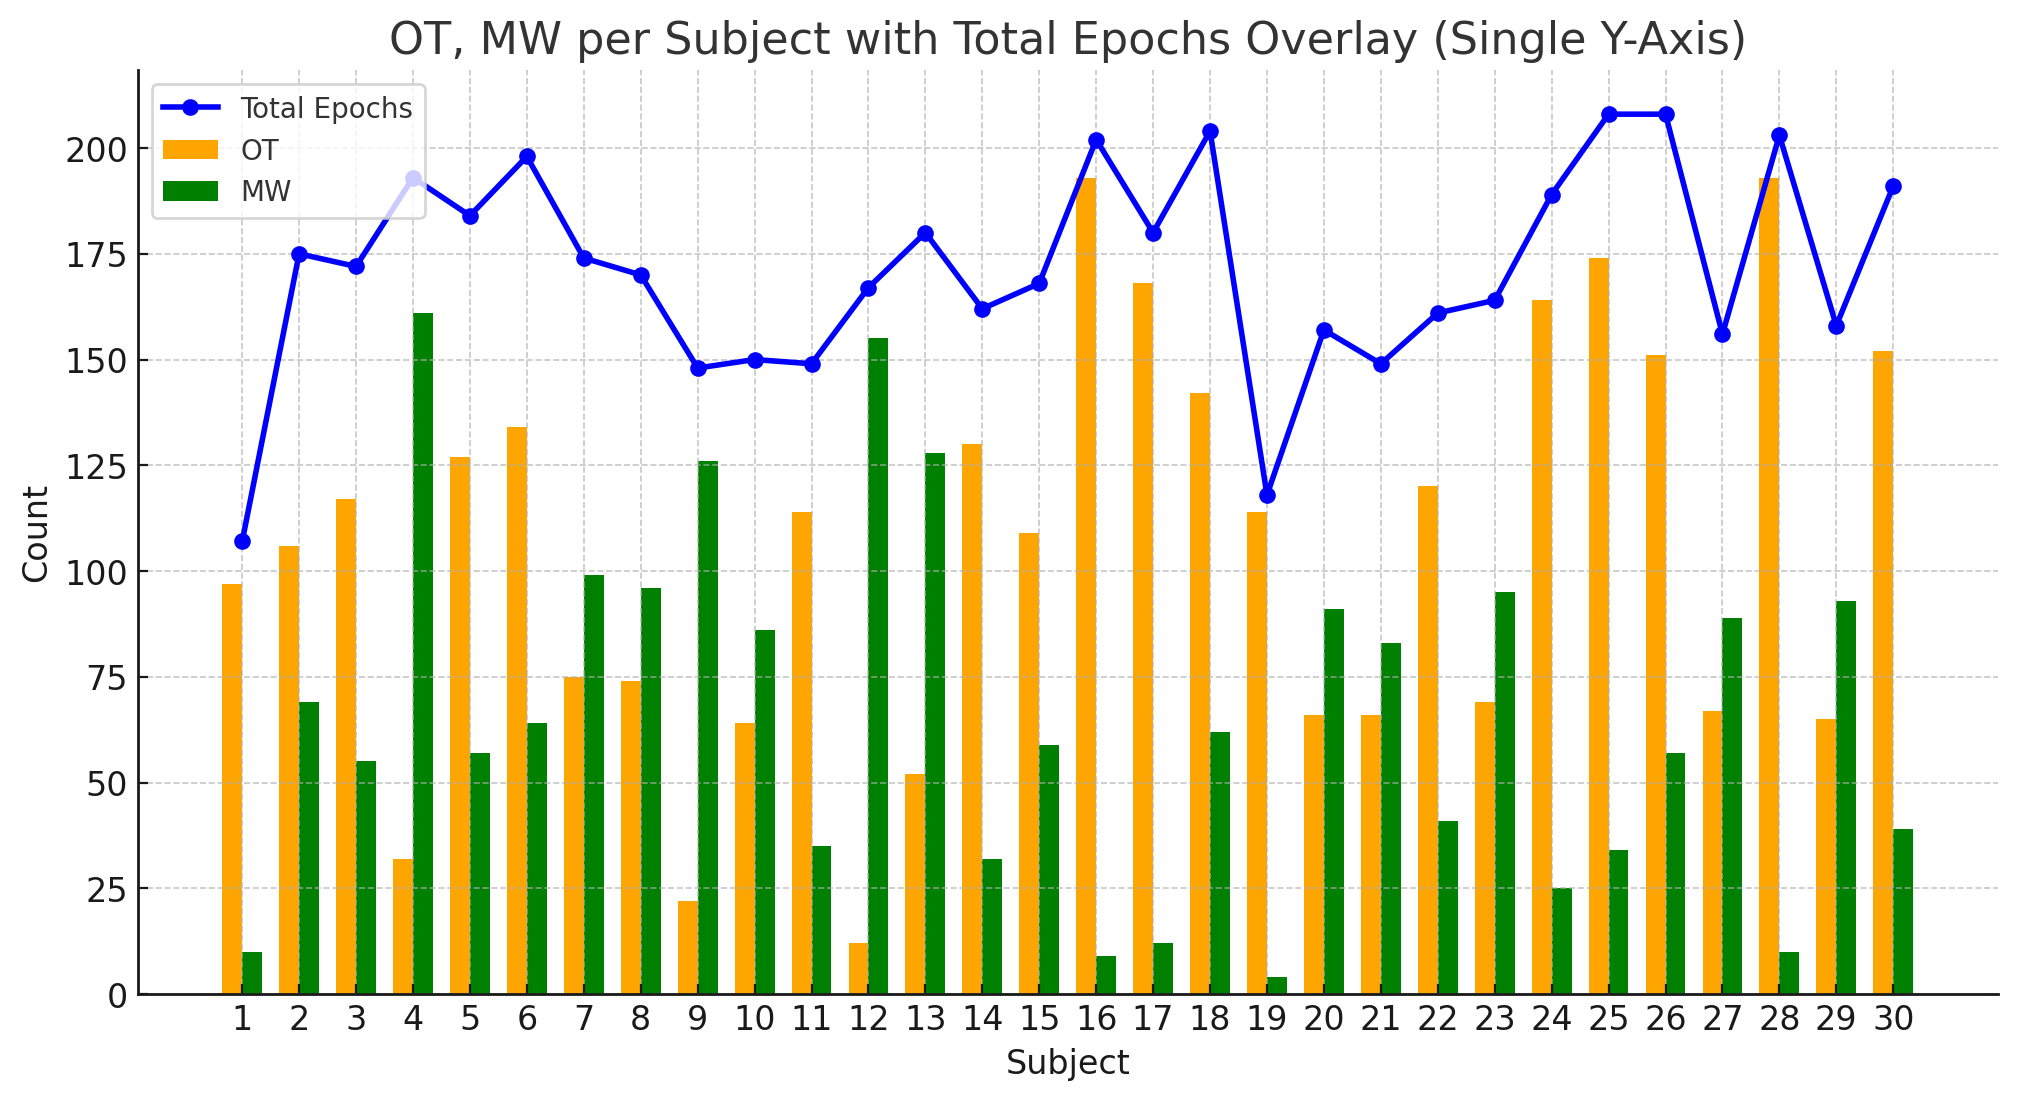
\includegraphics[width=400px]{Figures/dataset_dist.png}
    \caption{Distribution of Epochs for every subject.}
    \label{fig: dataset_dist}
\end{figure}
%\section{Project thesis study data analysis}
%
\section{PANAS}

Here are some preliminary results from the PANAS questionnaire. The response level was coded as shown in \autoref{responselvl}, leading to a maximum average of 4, a minimum average of 0, and a mean of 2.


\begin{table}[htbp] % Table of resppnslevel
    \centering
    \caption{Response Level Categories}
    \begin{tabular}{|c|c|}
        \hline
        \textbf{Response Level} & \textbf{Numerical Value} \\
        \hline
        Very slightly or not at all & 0 \\
        A little & 1 \\
        Moderately & 2 \\
        Quite a bit & 3 \\
        Extremely & 4 \\
        \hline
    \end{tabular}
    \label{responselvl}
\end{table} %Respons level Table

\begin{figure}
    \centering
    \includegraphics[width=350px]{Figures/panas/avarages/Positive-Emotions.png}
    \caption{Plot of the Avarage Total Positive Emotions trend by practice in the PANAS questionnaire throughout the protocol.}
    \label{fig:positive_by_practice}
\end{figure} % Positive Avarage
\begin{figure}
    \centering
    \includegraphics[width=350px]{Figures/panas/avarages/Negative-Emotions.png}
    \caption{Plot of the Avarage Total Negative Emotions trend by practice in the PANAS questionnaire throughout the protocol.}
    \label{fig:negative_by_practice}
\end{figure} % Negative Avarage



\begin{figure}
    \centering
    \begin{minipage}{0.49\linewidth}
        \includegraphics[width=\linewidth]{Figures/panas/emotions/Active.png}
        \caption{Plot of the Active emotion trend by practice in the PANAS questionnaire throughout the protocol.}
        \label{fig:active_by_practice}
    \end{minipage}
    \hfill % Adds horizontal space between the figures
    \begin{minipage}{0.49\linewidth}
        \includegraphics[width=\linewidth]{Figures/panas/emotions/Afraid.png}
        \caption{Plot of the Afraid emotion trend by practice in the PANAS questionnaire throughout the protocol.}
        \label{fig:afraid_by_practice}
    \end{minipage}
\end{figure} % Active and Afraid plots

\begin{figure}
    \centering
    \begin{minipage}{0.49\linewidth}
        \includegraphics[width=\linewidth]{Figures/panas/emotions/Alert.png}
        \caption{Plot of the Alert emotion trend by practice in the PANAS questionnaire throughout the protocol.}
        \label{fig:alert_by_practice}
    \end{minipage}
    \hfill % Adds horizontal space between the figures
    \begin{minipage}{0.49\linewidth}
        \includegraphics[width=\linewidth]{Figures/panas/emotions/Ashamed.png}
        \caption{Plot of the Ashamed emotion trend by practice in the PANAS questionnaire throughout the protocol.}
        \label{fig:ashamed_by_practice}
    \end{minipage}
\end{figure} % Alert and Ashamed plots

\begin{figure}
    \centering
    \begin{minipage}{0.49\linewidth}
        \includegraphics[width=\linewidth]{Figures/panas/emotions/Attentive.png}
        \caption{Plot of the Attentive emotion trend by practice in the PANAS questionnaire throughout the protocol.}
        \label{fig:attentive_by_practice}
    \end{minipage}
    \hfill % Adds horizontal space between the figures
    \begin{minipage}{0.49\linewidth}
        \includegraphics[width=\linewidth]{Figures/panas/emotions/Determined.png}
        \caption{Plot of the Determined emotion trend by practice in the PANAS questionnaire throughout the protocol.}
        \label{fig:Determined_by_practice}
    \end{minipage}
\end{figure} % Attentive and Determined plots

\begin{figure}
    \centering
    \begin{minipage}{0.49\linewidth}
        \includegraphics[width=\linewidth]{Figures/panas/emotions/Distressed.png}
        \caption{Plot of the Distressed emotion trend by practice in the PANAS questionnaire throughout the protocol.}
        \label{fig:distressed_by_practice}
    \end{minipage}
    \hfill % Adds horizontal space between the figures
    \begin{minipage}{0.49\linewidth}
        \includegraphics[width=\linewidth]{Figures/panas/emotions/Enthusiastic.png}
        \caption{Plot of the Enthusiastic emotion trend by practice in the PANAS questionnaire throughout the protocol.}
        \label{fig:enthusiastic_by_practice}
    \end{minipage}
\end{figure} % Distressed and Enthusiastic plots

\begin{figure}
    \centering
    \begin{minipage}{0.49\linewidth}
        \includegraphics[width=\linewidth]{Figures/panas/emotions/Excited.png}
        \caption{Plot of the Excited emotion trend by practice in the PANAS questionnaire throughout the protocol.}
        \label{fig:excited_by_practice}
    \end{minipage}
    \hfill % Adds horizontal space between the figures
    \begin{minipage}{0.49\linewidth}
        \includegraphics[width=\linewidth]{Figures/panas/emotions/Guilty.png}
        \caption{Plot of the Guilty emotion trend by practice in the PANAS questionnaire throughout the protocol.}
        \label{fig:guilty_by_practice}
    \end{minipage}
\end{figure} % Excited and Guilty plots

\begin{figure}
    \centering
    \begin{minipage}{0.49\linewidth}
        \includegraphics[width=\linewidth]{Figures/panas/emotions/Hostile.png}
        \caption{Plot of the Hostile emotion trend by practice in the PANAS questionnaire throughout the protocol.}
        \label{fig:hostile_by_practice}
    \end{minipage}
    \hfill % Adds horizontal space between the figures
    \begin{minipage}{0.49\linewidth}
        \includegraphics[width=\linewidth]{Figures/panas/emotions/Inspired.png}
        \caption{Plot of the Inspired emotion trend by practice in the PANAS questionnaire throughout the protocol.}
        \label{fig:inspired_by_practice}
    \end{minipage}
\end{figure} % Hostile and Inspired plots

\begin{figure}
    \centering
    \begin{minipage}{0.49\linewidth}
        \includegraphics[width=\linewidth]{Figures/panas/emotions/Interested.png}
        \caption{Plot of the Interested emotion trend by practice in the PANAS questionnaire throughout the protocol.}
        \label{fig:interested_by_practice}
    \end{minipage}
    \hfill % Adds horizontal space between the figures
    \begin{minipage}{0.49\linewidth}
        \includegraphics[width=\linewidth]{Figures/panas/emotions/Irritable.png}
        \caption{Plot of the Irritable emotion trend by practice in the PANAS questionnaire throughout the protocol.}
        \label{fig:irritable_by_practice}
    \end{minipage}
\end{figure} % Interesed and Irritable plots

\begin{figure}
    \centering
    \begin{minipage}{0.49\linewidth}
        \includegraphics[width=\linewidth]{Figures/panas/emotions/Jittery.png}
        \caption{Plot of the Jittery emotion trend by practice in the PANAS questionnaire throughout the protocol.}
        \label{fig:jittery_by_practice}
    \end{minipage}
    \hfill % Adds horizontal space between the figures
    \begin{minipage}{0.49\linewidth}
        \includegraphics[width=\linewidth]{Figures/panas/emotions/Nervous.png}
        \caption{Plot of the Nervous emotion trend by practice in the PANAS questionnaire throughout the protocol.}
        \label{fig:nervous_by_practice}
    \end{minipage}
\end{figure} % Jittery and Nervous plots

\begin{figure}
    \centering
    \begin{minipage}{0.49\linewidth}
        \includegraphics[width=\linewidth]{Figures/panas/emotions/Proud.png}
        \caption{Plot of the Proud emotion trend by practice in the PANAS questionnaire throughout the protocol.}
        \label{fig:proud_by_practice}
    \end{minipage}
    \hfill % Adds horizontal space between the figures
    \begin{minipage}{0.49\linewidth}
        \includegraphics[width=\linewidth]{Figures/panas/emotions/Scared.png}
        \caption{Plot of the Scared emotion trend by practice in the PANAS questionnaire throughout the protocol.}
        \label{fig:scared_by_practice}
    \end{minipage}
\end{figure} % Proud and Scared plots

\begin{figure}
    \centering
    \begin{minipage}{0.49\linewidth}
        \includegraphics[width=\linewidth]{Figures/panas/emotions/Strong.png}
        \caption{Plot of the Strong emotion trend by practice in the PANAS questionnaire throughout the protocol.}
        \label{fig:strong_by_practice}
    \end{minipage}
    \hfill % Adds horizontal space between the figures
    \begin{minipage}{0.49\linewidth}
        \includegraphics[width=\linewidth]{Figures/panas/emotions/Upset.png}
        \caption{Plot of the Upset emotion trend by practice in the PANAS questionnaire throughout the protocol.}
        \label{fig:upset_by_practice}
    \end{minipage}
\end{figure} % Strong and Upset plots
%\section{State Anxiety Inventory}
%\section{Trait Anxiety Inventory}
%\section{PROMIS}